% % % Beginning of preamble...
\documentclass[10pt,a4paper]{report}

% % % packages to be used...
\usepackage[utf8]{inputenc}
\usepackage[english]{babel}
\usepackage{amsmath}
\usepackage{amsfonts}
\usepackage{amssymb}
\usepackage{graphicx}
\usepackage{lineno}
\usepackage{subfig}
\usepackage{caption}
\usepackage{enumerate}
\usepackage{graphicx}
\usepackage{float}
\usepackage{array}
\usepackage{fancyhdr}
\usepackage[left=2.50cm, right=2.50cm, top=2.50cm, bottom=2.50cm]{geometry}

% % % Document data...
\author{Yasiel Delabat Diaz}
\title{}


% % % Define the syles....
\fancypagestyle{chapter-first-page}{
	\fancyhf{}
	\fancyhead[R]{\thepage}
	\fancyhead[C]{}
	\fancyhead[L]{}
	\fancyfoot[R]{}
	\fancyfoot[C]{[DRAFT]}
	\fancyfoot[L]{}
}
\fancypagestyle{introduction}{
	\fancyhf{}
	\fancyhead[R]{}
	\fancyhead[C]{}
	\fancyhead[L]{Introduction}
	\fancyfoot[R]{}
	\fancyfoot[C]{[DRAFT]}
	\fancyfoot[L]{}
}
\fancypagestyle{standard}{
	\fancyhf{}
	\fancyhead[R]{\thepage}
	\fancyhead[C]{}
	\fancyhead[L]{\nouppercase{\leftmark}}
	\fancyfoot[R]{}
	\fancyfoot[C]{[DRAFT]}
	\fancyfoot[L]{}
}
\fancypagestyle{conclusions}{
	\fancyhf{}
	\fancyhead[R]{}
	\fancyhead[C]{}
	\fancyhead[L]{Conclusions}
	\fancyfoot[R]{}
	\fancyfoot[C]{[DRAFT]}
	\fancyfoot[L]{}
}
\fancypagestyle{references}{
	\fancyhf{}
	\fancyhead[R]{}
	\fancyhead[C]{}
	\fancyhead[L]{References}
	\fancyfoot[R]{}
	\fancyfoot[C]{[DRAFT]}
	\fancyfoot[L]{}
}

% % % Show line numbers (for DRAFT version)
\linenumbers

% % % New table columns alignment option:
\newcolumntype{P}[1]{>{\centering\arraybackslash}p{#1}}

% % % Beginning of document...
\begin{document}

	% % % Add the different parts here...
	% % % Set the style for this file:
\pagestyle{introduction}

% % % Beginning of the section
\section*{\uppercase{Introduction}}\label{intro}
	\bigskip
	\bigskip
	Petals are the local support structures holding the ATLAS end-cap ITk strip sensors \ref{ref1}. For the petal sensors, a series of tests are being designed to cover both Quality Assurance (QA) and Quality Control (QC). These include a series of tests on their assembled structure (through metrology surveys), their electrical functionality and their thermomechanical properties (including ASIC burn in, thermal cycling and long term cold tests). 
	As it’s very important that, during the QC process, good care is taken not to damage the fragile components of the sensors, the thermal tests will be made by using infrared thermography, which is the most suitable technique to employ for this purposes. However, depending on the target surface, infrared measurements can be quite inaccurate and unreliable. Silicon, for example, is a tricky material to perform infrared measures on, and it’s however the most important component on the detector sensors. That is why a good understanding of infrared thermography is crucial to achieve accurate temperature measurements.
	For simulating the sensor's response at different operational parameters, thermal Finite Element Analyses (FEAs) are used. In particular, for the petal FEA models, exact design specifications of each component are considered. However, this simulation model have to be validated. For that purpose, numerous building institutes assembled and measured thermo-mechanical module prototypes. 
	In this study, we use the thermomechanical petal prototype assembled at DESY aiming at two main objectives: to contribute to the improvement of the QC and QA processes of the petal structures for the ATLAS end-caps and to perform infrared tests on the current petal thermomechanical prototype in order to provide the FEA team with a comparison point to validate their model. In order to do so, a reliable IR temperature determination is indispensable. To that end, a series of studies were performed to gain better understanding of the way in which those factors affect such measurements:
		
	\begin{enumerate}
		\item Apparent reflected temperature determination.
		\item IR camera’s intrinsic spectral response scale factor determination.
		\item Emissivity correction/estimation methods for the silicon sensors.
		\item Viewing angle influence.
	\end{enumerate}
	
	This report contains the results of these studies and is structured as follows: In Chapter 1 a brief background on infrared thermography, needed for the subsequent sections is given. In Chapter 2 a detailed description of the experimental setup used in this work is presented. In Chapter 3, the analysis methods used in the different studies is discussed. Finally, in Chapter 4, the results are presented accompanied by a small discussion. 
	\clearpage
	
	\chapter{Notions of infrared thermography}

	\section{Infrared radiation spectrum.}
	
		Infrared (IR) radiation is the energy irradiated by a surface that has a temperature above the absolute zero [1]. Within the electromagnetic spectrum, IR radiation is defined as the radiation band that spans from 0.7 $\mu$m to 1000 $\mu$m in wavelength (Figure \ref{fig1}).\\ Much of the IR spectrum, however, is not useful for Infrared thermography (IRT) due to atmospheric absorption. This absorption occurs mainly with $H_{2}O$ and $CO_{2}$ molecules as they are well known for being good heat absorbers (Figure \ref{fig2}). According to this fact, the IR wavelength range is sometimes further divided into 4 additional categories:

		\begin{enumerate}[I.]
			\item Near-infrared (NIR) from 0.8 $\mu$m to 1.7 $\mu$m.
			\item Short-wavelength infrared (SWIR) from 1 $\mu$m to 2.5 $\mu$m.
			\item Mid-wavelength infrared (MWIR) from 2 $\mu$mm to 5 $\mu$mm.
			\item Long-wavelength infrared (LWIR) from 8 $\mu$mm to 14 $\mu$mm.
		\end{enumerate}
		
		\begin{figure}[ht!]
			\centering
			\captionsetup{justification=centering,margin=2cm}
			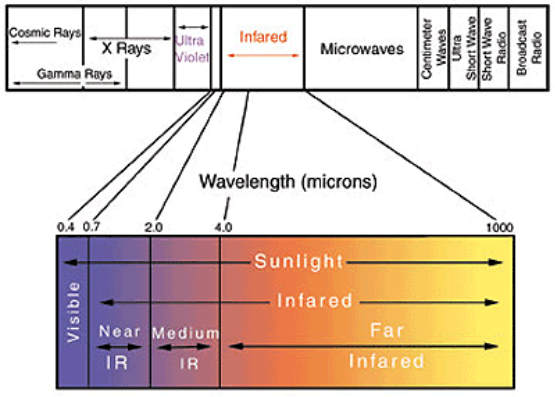
\includegraphics[scale=0.75]{Figures/Chapter01/lightspectrum}
			\caption{\label{fig1} Electromagnetic spectrum showing the portion corresponding to IR radiation.}
		\end{figure}
		
		It is important to note that this classification is somewhat arbitrary and therefore it can change quite a bit from one author to the other but in general they remain fairly similar. Most IR sensors are designed to work in the LWIR part of the spectrum since this is the range that minimizes this absorptions.\\ In this study, as we use an IR camera sensitive only to the fourth type, we will refer to IR as the LWIR except otherwise explicitly stated.
		
		\begin{figure}[ht!]
			\centering
			\captionsetup{justification=centering,margin=2cm}
			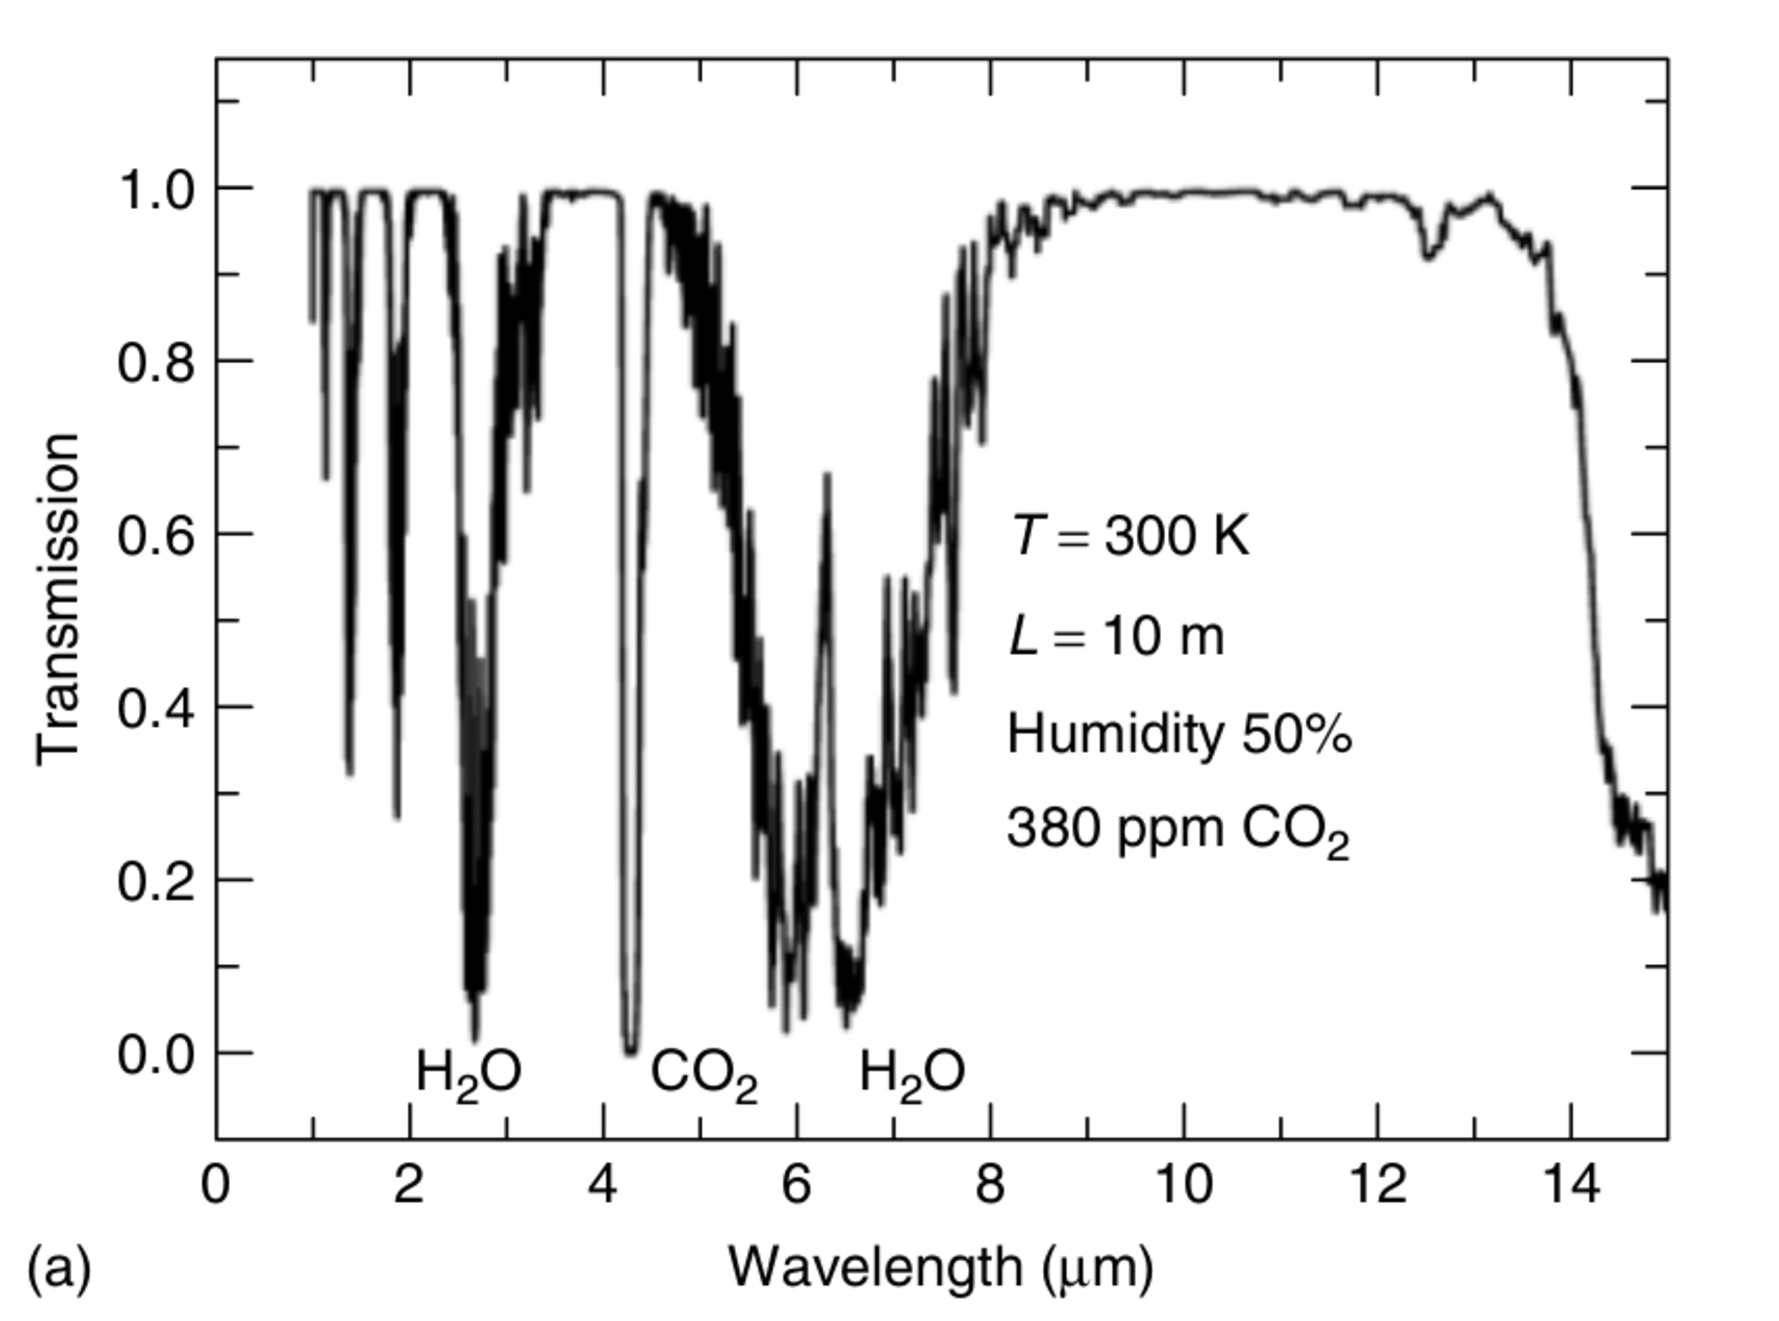
\includegraphics[scale=0.45]{Figures/Chapter01/Transmission.pdf}
			\caption{\label{fig2} A typical atmospheric transmittance plot  for infrared radiation. For some of the minima we can see the absorbing molecule responsible,}
		\end{figure}
		
	\section{Plank's law for blackbodies. IR radiation dissipation.}
	
		According to Plank's law, the IR emissive power of a blackbody at a temperature $T$, with a wavelength between $\lambda$ and $\lambda+d\lambda$ is given by equation (\ref{eq1}), where $C_{1}$ and $C_{2}$ are constants, often called first and second radiation constants respectively [2].
		
		\begin{equation}
			\label{eq1}
			N_{b}(\lambda,T)d\lambda=\frac{C_{1} \cdot \lambda^{-5}}{\exp (\frac{C_{2}}{\lambda\cdot T}) -1} d\lambda
		\end{equation}
		
		Figure \ref{fig3} shows this functional dependence for six different temperatures [3]. The gray line represents the displacement of the maximum for each temperature. Note that, as the temperature decreases, the maximum emissive power moves to higher wavelengths, this is known as the Wien's displacement law [4]. 
		
		There are three ways by which the emissive power striking an object may be dissipated: absorption, transmission and reflection [5]. The fractions of the total radiant energy that are associated with each of these modes of dissipation are referred to as the \textit{absorptivity}, \textit{transmissivity} and \textit{reflectivity} of the body. Three parameters are used to describe these phenomena: the spectral \textit{absorptance} $\alpha$, which is the fraction of the spectral emissive power absorbed by the object, the spectral \textit{reflectance} $\rho$, which is the fraction of the spectral emissive power reflected by the object, and the spectral \textit{transmittance} $\tau$, which is the fraction of the spectral emissive power transmitted by the object.
		
		\begin{figure}[ht!]
			\centering
			\captionsetup{justification=centering,margin=2cm}
			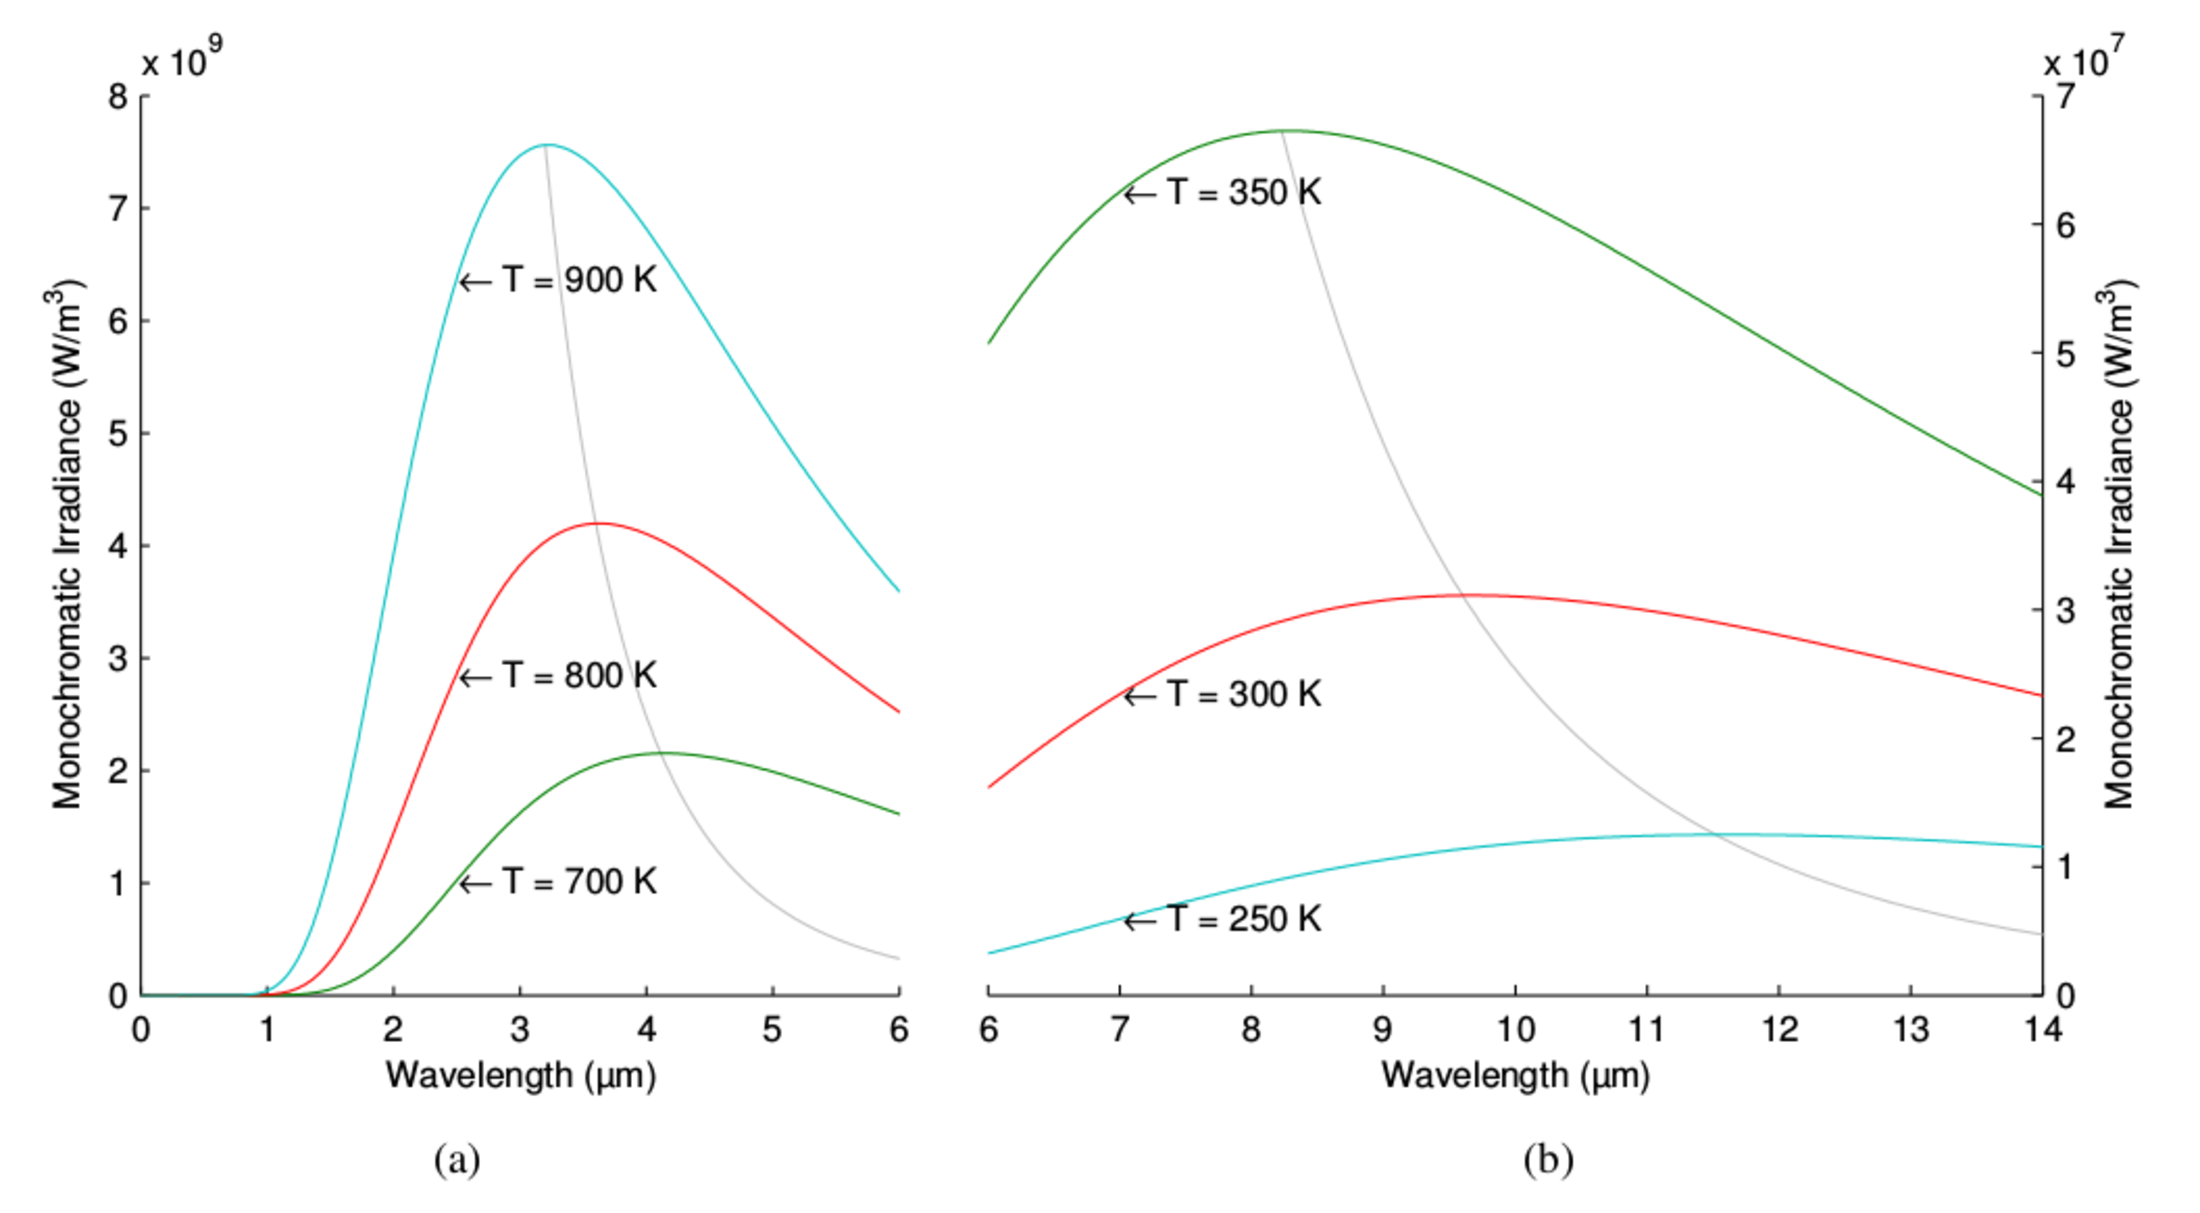
\includegraphics[scale=0.45]{Figures/Chapter01/PlankFunction.pdf}
			\caption{\label{fig3} Planck's law: electromagnetic radiation emitted by a blackbody in thermal equilibrium at a definite  temperature. (a) Objects with a high temperature emit most of the radiation in the middle wave infrared; (b) Objects with a low temperature emit most of the radiation in the long wave infrared. The two parts of the graph are scaled differently on the y-axis.}
		\end{figure}		
		
		These three parameters are, in general, wavelength dependent and their sum must be one at any given wavelength and surface temperature:
		
		\begin{equation}
			\label{eq2}
			\alpha + \rho + \tau = 1
		\end{equation}	
		
			
	\clearpage
	
	% % % Set the style for this file:
\pagestyle{standard}

% % % Beginning of the chapter
\chapter{Experimental setup}\label{chapter2}

	% % % Set the style for the first page:
	\thispagestyle{chapter-first-page}
	
	\section{Thermo-mechanical Petal}\label{section2.1}
	
		Both ATLAS ITk strip end-caps (Figure \ref{fig2.1} left) are composed by 6 disks which individually can hold 32 other local support structures called petals (Figure \ref{fig2.1} right). The petal structure is the frame where the end-cap sensors are mounted. It provides the mechanical support needed by the sensors as well as the electronics and cooling services. Each petal holds 9 sensors (Figure \ref{fig2.1} right). For the ATLAS Phase-II upgrade new Petal design is still under development. However, in this study a thermo-mechanical prototype build partially by hand is used, equipped with dummy electronics modules, blank silicon wafers and mechanical components to be a thermal equivalent to the final structure. As the petal’s design is still being improved, our prototype became quickly “obsolete”. In fact, some key materials for IR studies in the current prototype such as the silicon wafers are not very IR friendly because of their high transmissivity. This makes really difficult the employment of non-contact temperature measuring methods (See Chapter \ref{chapter3}). In contrast, newer silicon wafers are available which are not transmissive.
				
		\begin{figure}[ht!]
			\centering
			\captionsetup{justification=centering,margin=2cm}
			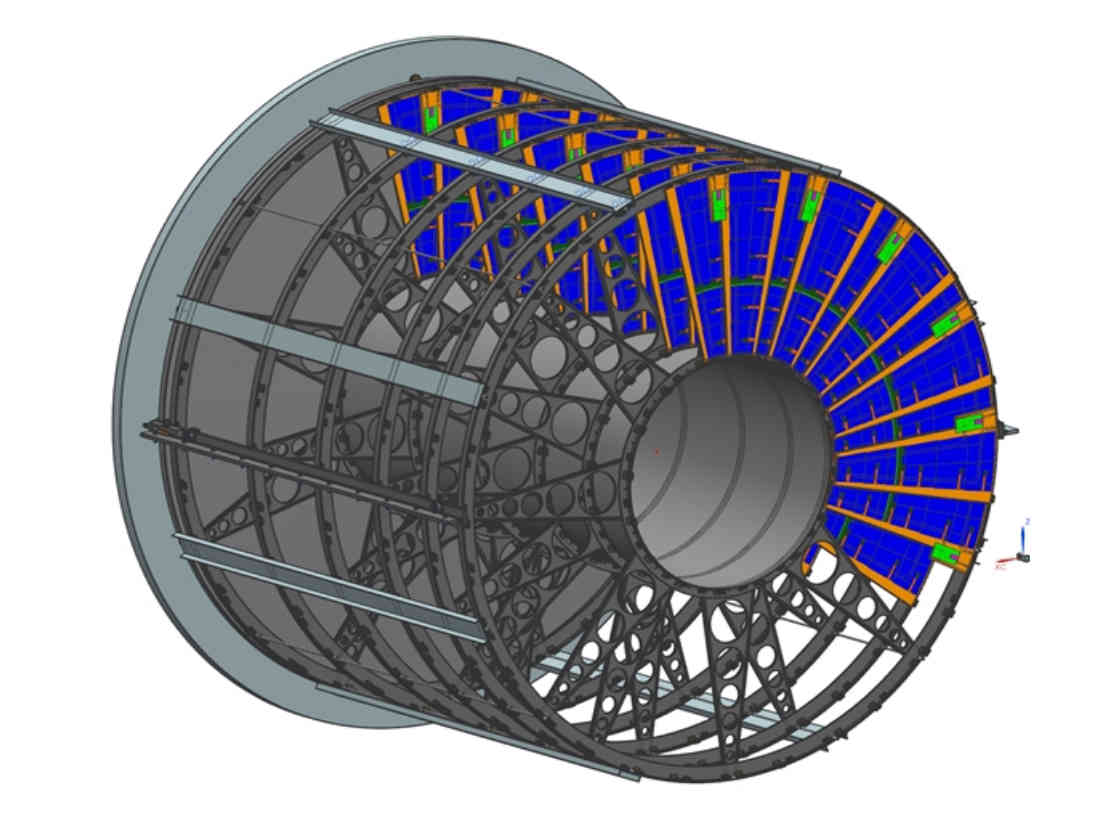
\includegraphics[scale=0.25]{Figures/Chapter02/EndCap.jpg}
			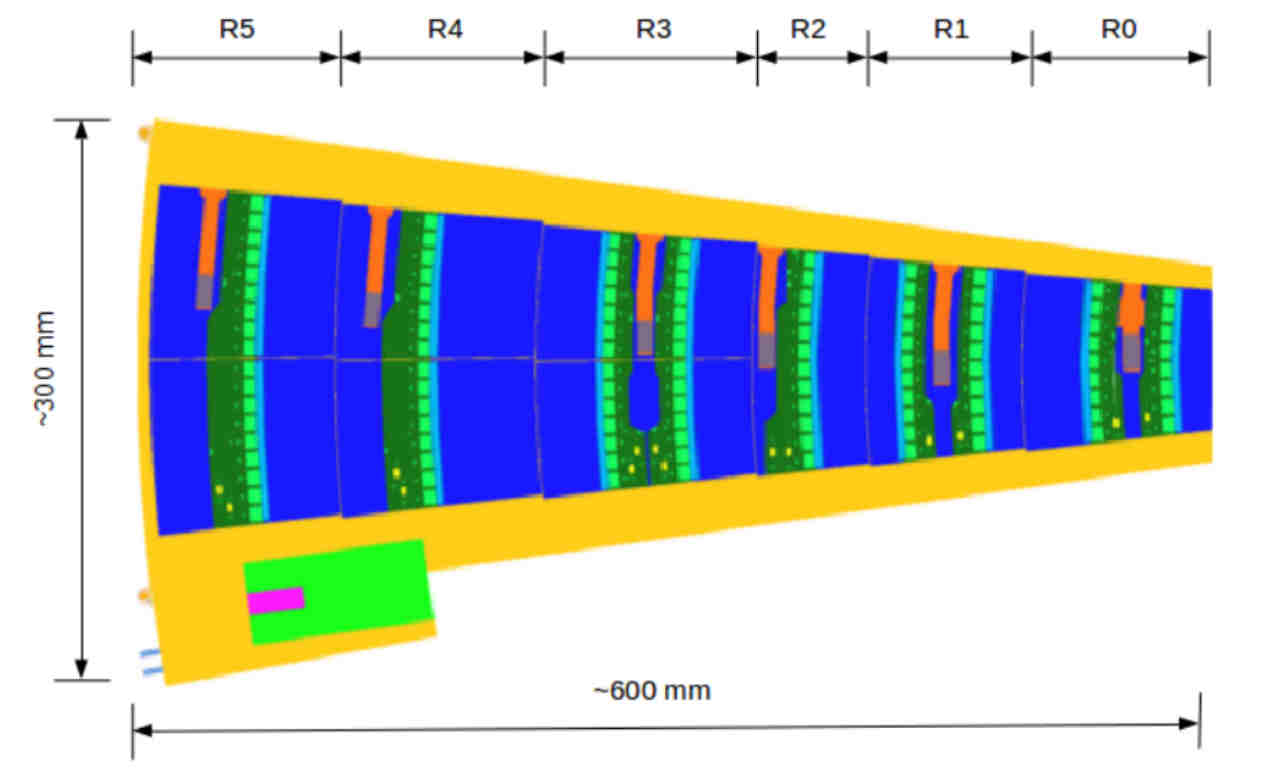
\includegraphics[scale=0.26]{Figures/Chapter02/PetalDesign.jpg}
			\caption{ATLAS strip detector end-cap (left) showing petal structures and a schematic view of the petal showing the 6 different modules (right).}\label{fig2.1}
		\end{figure}
		
		The 6 petal modules are named R0 (closest to the beamline in the radial direction), R1, R2, R3, R4 and R5 . Each module contains, in general, the following components:
		
		\begin{itemize}
			\renewcommand{\labelitemi}{$\diamond$}
			\item Blank Si, laser cut (320 $\mu$m thick).
			\item FR4 PCBs (200 $\mu$m thick).
			\item Glass ASICs with heater pattern and bonding pads, glued with UV glue, wire-bonded to bare silicon.
			\item Real DC-DC converters, based on commercial LTC360 ASIC on a custom board.
			\item Potentiometer to adjust power input/output.
			\begin{itemize}
			\renewcommand{\labelitemi}{$\bullet$}
				\item Powered through bus tape power lines.
			\end{itemize}
			\item In the case of R0 module: v0 assembly tools, real hybrids, glass ASICs.
		\end{itemize}
		
		In addition, the prototype core was built using real materials with respect to preliminary petal designs (bus tape, honeycomb, Ti V-shaped cooling pipe), real copper power traces, dummy data-lines, and a dummy EoS (not present initially but recently installed) per side. Some of the above mentioned components can be seen in the Figure \ref{fig2.2}.
		
		\begin{figure}[ht!]
			\centering
			\captionsetup{justification=centering,margin=2cm}
			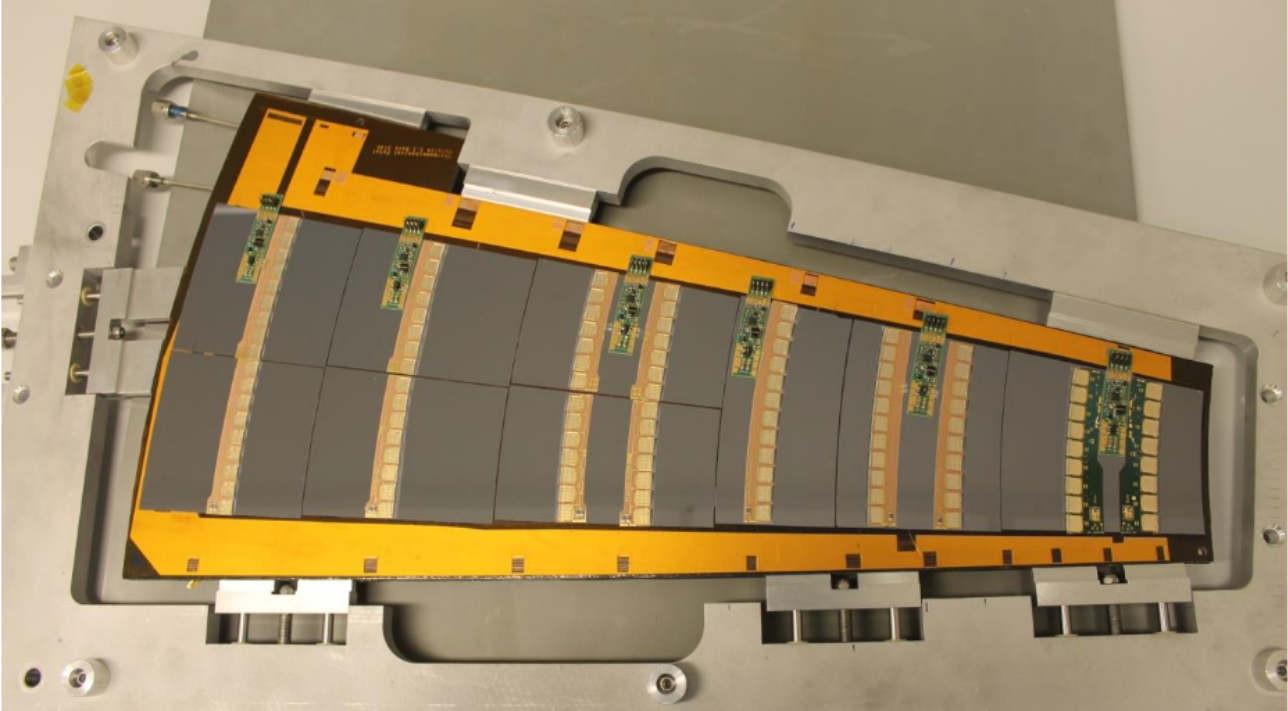
\includegraphics[scale=0.35]{Figures/Chapter02/PetalConstruction.jpg}
			\caption{Thermomechanical prototype of the Petal  used in the IR measurements.}\label{fig2.2}
		\end{figure}\bigskip
		
	\section{Custom Thermal Chamber. }\label{section2.2}
	
		For the infrared measurements, the thermomechanical petal prototype was placed inside a customised thermal chamber where, on one end, the petal is vertically inserted in a custom rail system (Figure \ref{fig2.3} left) and on the opposite end the IR camera is mounted on a mobile platform that can move horizontally and vertically thanks to an Arduino controlled Gantry System (Figure \ref{fig2.3} right). Temperature and relative humidity (RH) inside the chamber are monitored using three SHT21 sensors connected  to a Raspberry Pi. 
		
		\begin{figure}[ht!]
			\centering
			\captionsetup{justification=centering,margin=2cm}
			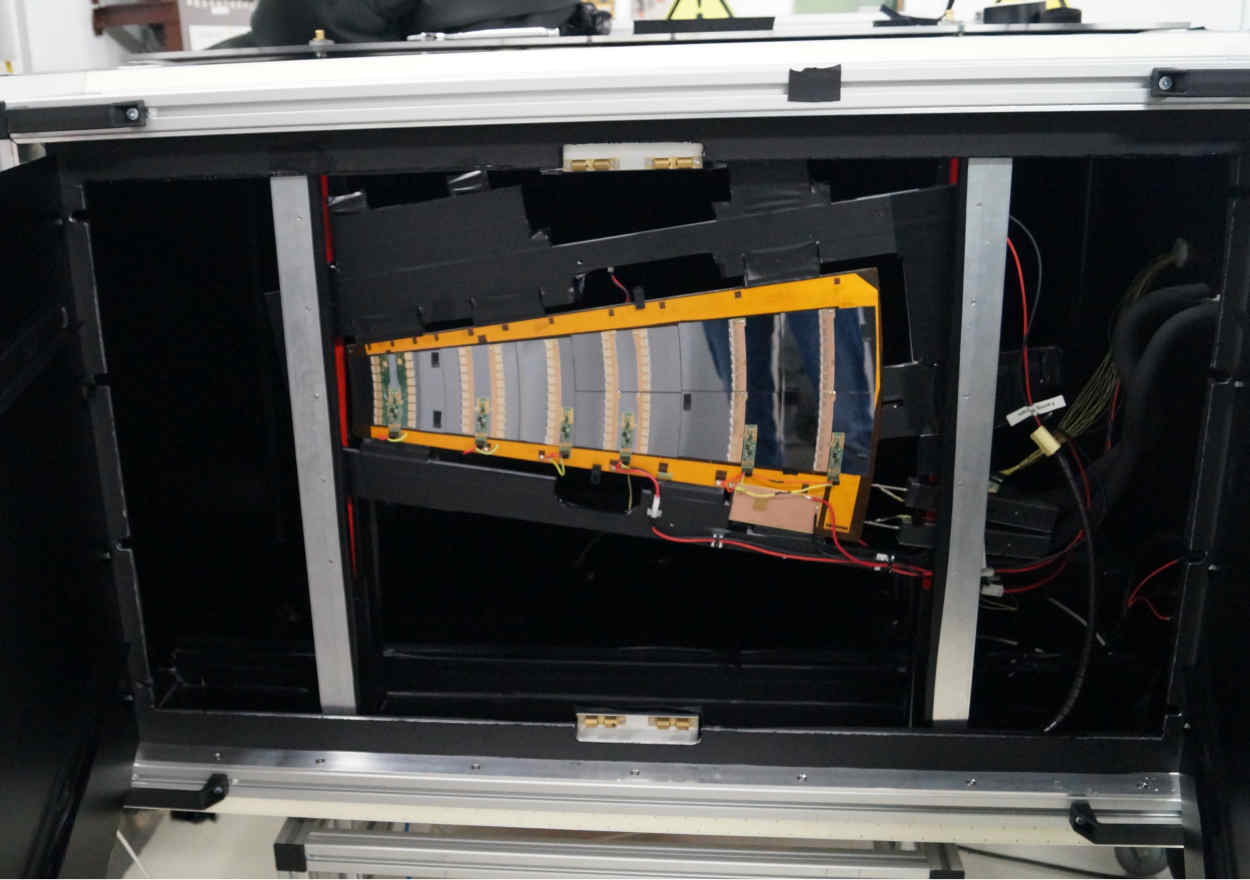
\includegraphics[scale=0.25]{Figures/Chapter02/ChamberBack.jpg}
			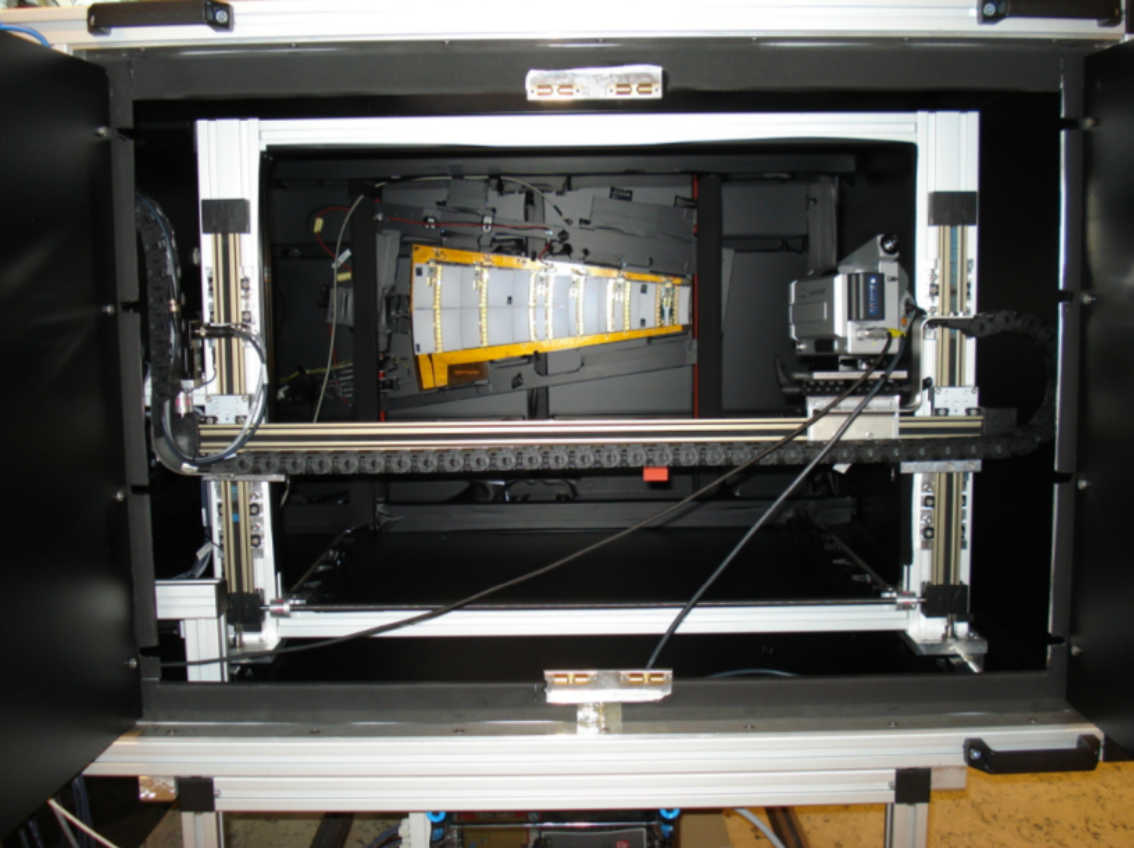
\includegraphics[scale=0.26]{Figures/Chapter02/CamberFront.jpg}
			\caption{Image of both ends of the thermal chamber showing the Petal already in place and the IR camera also in position.}\label{fig2.3}
		\end{figure}
		
		The use of the chamber has two main advantages: first, it provides shielding for the object under investigation against external heat sources such as ceiling lamps, computers and other electronic devices used in the setup; second, it is used as an enclosure where we can flush nitrogen in order to reduce the moisture and in doing so preventing condensation from ambient air on the cooled sensors, which would irreversibly damage the prototype. Low RH comes with the additional bonus of reducing the potential absorption of IR radiation in the air path from the target to the IR camera as discussed in Section \ref{section1.1}.
		In order to perform the IR measurements and avoid registering the heat from the camera that is reflected back by the petal surface\footnote{{\footnotesize This is known as Narcissus effect and it is an important source of background for the IR measurements if it’s not properly handled.}}, the IR camera is positioned in the chamber in such a way that it faces the Petal with an angle of incidence (Figure \ref{fig2.4}).	
		
		\begin{figure}[ht!]
			\centering
			\captionsetup{justification=centering,margin=2cm}
			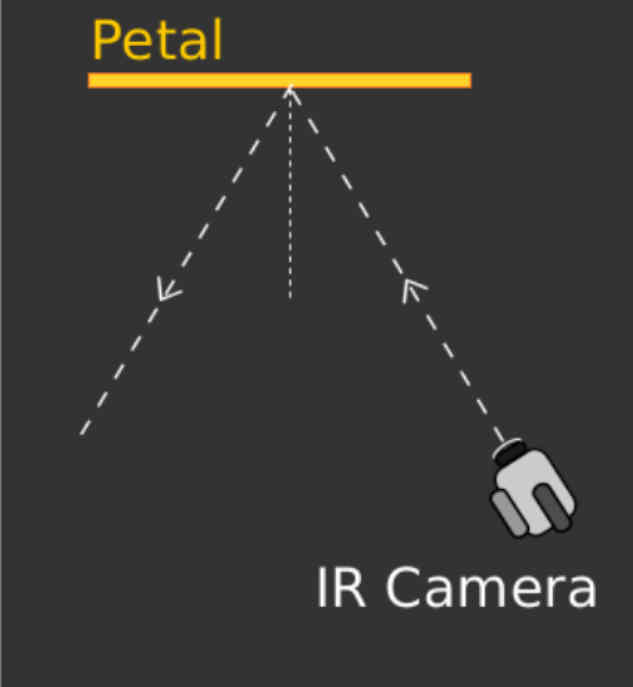
\includegraphics[scale=0.25]{Figures/Chapter02/NarcissusEffect.jpg}
			\caption{The IR camera is placed at some angle with respect to the plane of the petal to avoid the Narcissus effect.}\label{fig2.4}
		\end{figure}\bigskip
		
	\section{IR camera.}\label{section2.3}
	
		For this study a VarioCAM High Resolution (hr) IR camera from InfraTec GmbH was used (Figure \ref{fig2.5}). The VarioCAM $\textregistered$ hr is a thermographic system for the long wave infrared spectral range of 7.5 $\mu$m to 14 $\mu$m (LWIR). The lens images the object scene onto a microbolometer array at a resolution of 640 x 480 pixels. The electrical signal of the detector arrays is further processed by the internal electronics which basically consists in transforming the modified pixel resistance due to the incoming radiation into temperature. The electronics also contains all the functions necessary for camera operation, such as activation of the microbolometer array, A/D conversion, offset and gain correction, defective pixel treatment, video and PC interfaces \ref{ref9}.
		
		\begin{table}[ht!]
    		\begin{minipage}[b]{0.4\linewidth}
  				\centering
  				\captionsetup{justification=centering, margin=0.5cm}
  				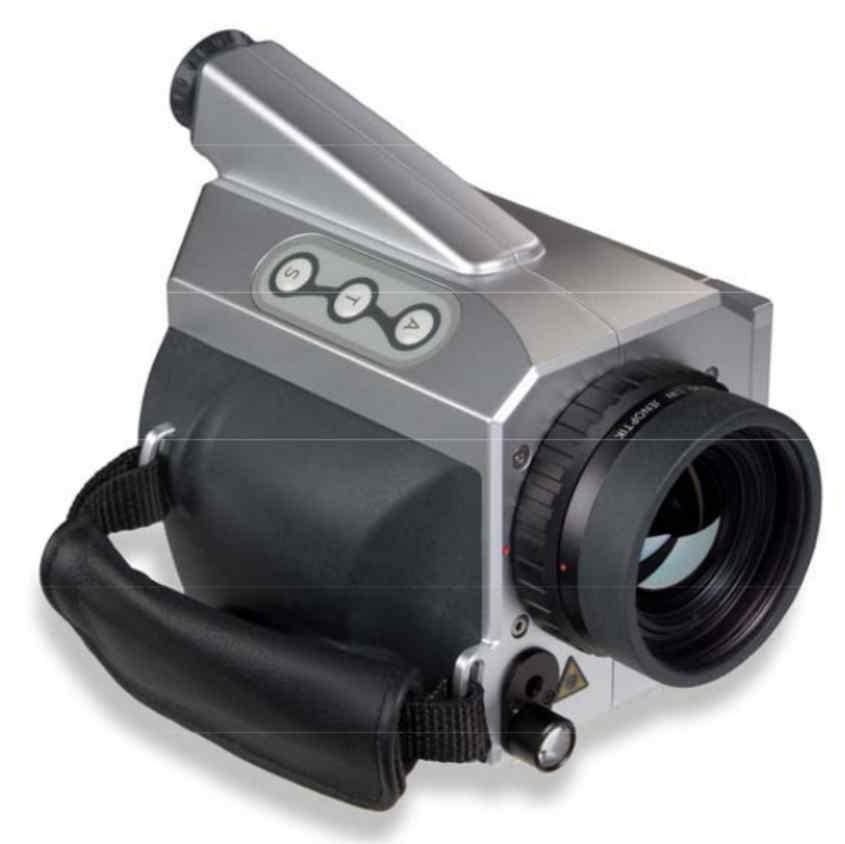
\includegraphics[scale=0.3]{Figures/Chapter02/PictureOfIRCamera.jpg}
  				\captionof{figure}{VarioCAM \textregistered\space hr (640 x 480 pixels) IR camera  from InfraTec \textcopyright\space GmbH.}\label{fig2.5}
    		\end{minipage}
    		\begin{minipage}[b]{0.7\linewidth}
    			\centering
  				\captionsetup{justification=raggedright}
        		\caption{VArioCam hr technical data.}\label{tab2.1}
				\begin{tabular}{p{0.35\linewidth}p{0.35\linewidth}}\hline
					\textbf{Temperature measuring range} & (-40 ... 1.200) $^{\circ}C$, optional $>$ 2.000 $^{\circ}C$ \\ \hline 
					\textbf{Temperature resolution @ 30 $^{\circ}C$} &  better than 0.08 K, up to 0.05 K (premium mode) \\ \hline
					\textbf{Emissivity} & Adjustable from 0.1 to 1.0, in increments of 0.01 \\ \hline
					\textbf{Detector} &  uncooled microbolometer Focal Plane Array \\ \hline
					\textbf{A/D conversion} &  16 bit \\ \hline 
					\textbf{Operation temperature} & (-15 ... 50) $^{\circ}C$ \\ \hline
					\textbf{Humidity during operation and storage} & 5\% to 95\%, non-condensing \\ \hline
					\textbf{Shock resistance} & 25 G, IEC 68-2-29 \\ \hline
				\end{tabular}
    		\end{minipage}
		\end{table}
		
		The camera’s accuracy for temperature measurement (reported by manufacturer) is $\pm 1.5 K$ in the range from 0\space$^\circ C$ to 100\space$^\circ C$ and $\pm2$\% anywhere outside that range. Some additional technical data is presented in Table \ref{tab2.1}.
		
		The data acquisition is performed using the VarioCam hr control software IRBIS $\textregistered$ professional v3.1 (Figure \ref{fig2.6}). Each image is computed as an average of 100 acquisitions regularly taken during five seconds in order to reduce uncertainty due to pixels noise. All thermograms are recorded in units of absolute temperature (K) and emissive power ($W/m^2$) for further offline analysis.
		
		\begin{figure}[ht!]
			\centering
			\captionsetup{justification=centering,margin=2cm}
			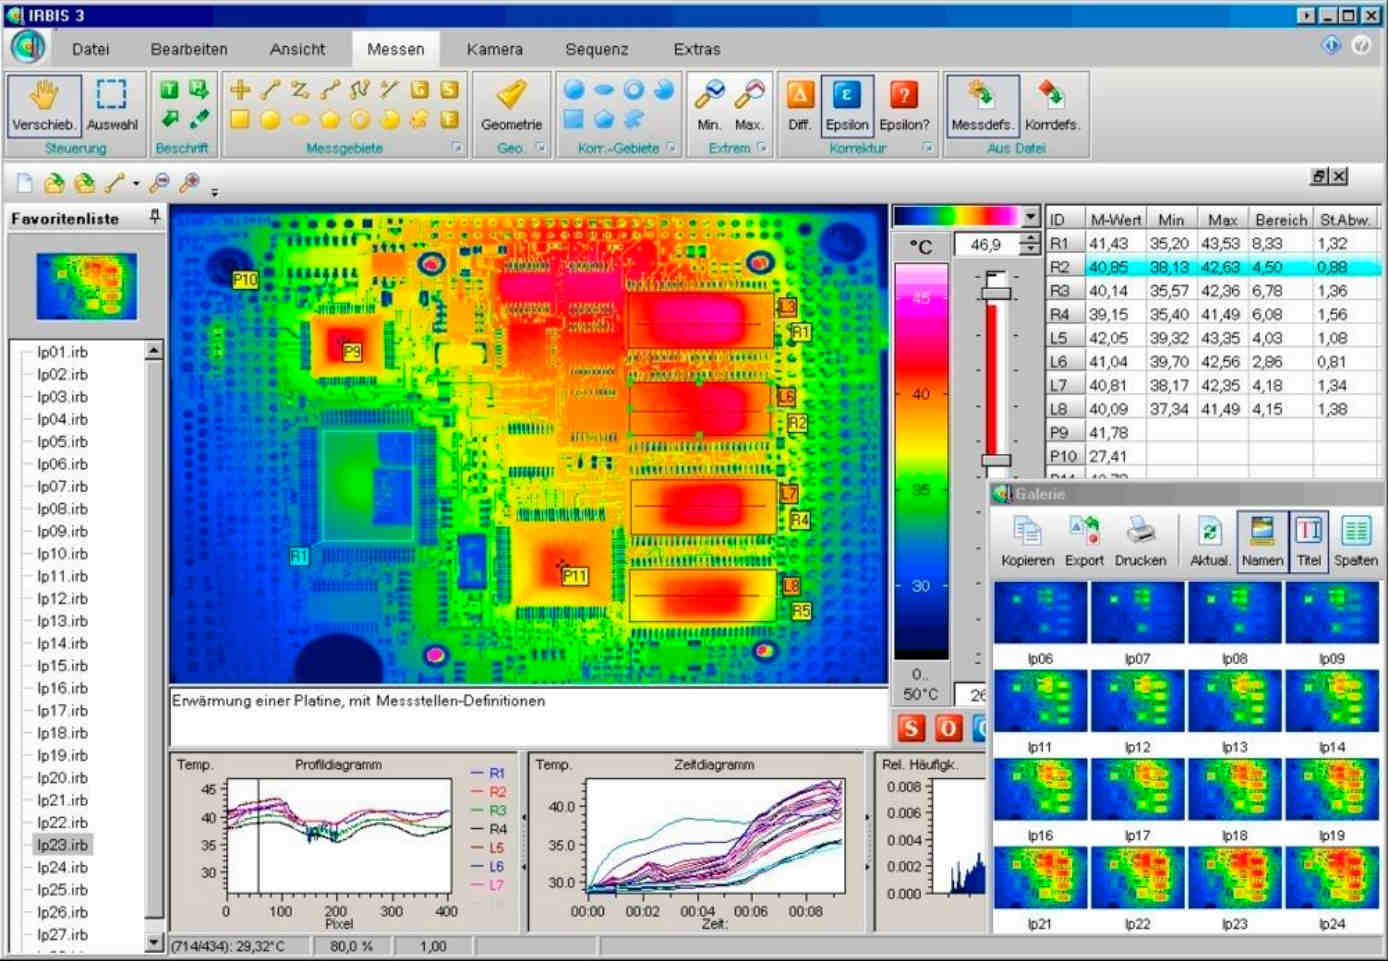
\includegraphics[scale=0.25]{Figures/Chapter02/IRBISimage.jpg}
			\caption{Screenshot of the camera’s control software IRBIS $\textregistered$ 3.1.}\label{fig2.6}
		\end{figure}\bigskip
		
	\section{Setup configuration.}\label{section2.4}
	
		In this study, two thermal cycles performed using the setup described below are considered, corresponding to both sides of the Petal and measured with the latest experimental configuration. In the following, this will be referred to as “cycle 2” (unpolished side) and “cycle 9” (polished side) in allusion to the dates in which the measurements began (August 2nd and August 9th, 2017). 
		
		Much of the improvements of the experimental setup came from experiences of preliminary tests when we realized that, for example, the heat from the Gantry system was being reflected on the Petal’s surface and registered by the IR camera. Thus, a curtain from an IR opaque black fabric was placed between the Petal and the Gantry system (leaving a small hole for the camera lens) to suppress this effect (Figure \ref{fig2.7} right). In addition, other improvements to the chamber’s insulation were made to better control the ambient conditions inside at lower temperatures (Figure \ref{fig2.7} left). 
	
		\begin{figure}[ht!]
			\centering
			\captionsetup{justification=centering,margin=2cm}
			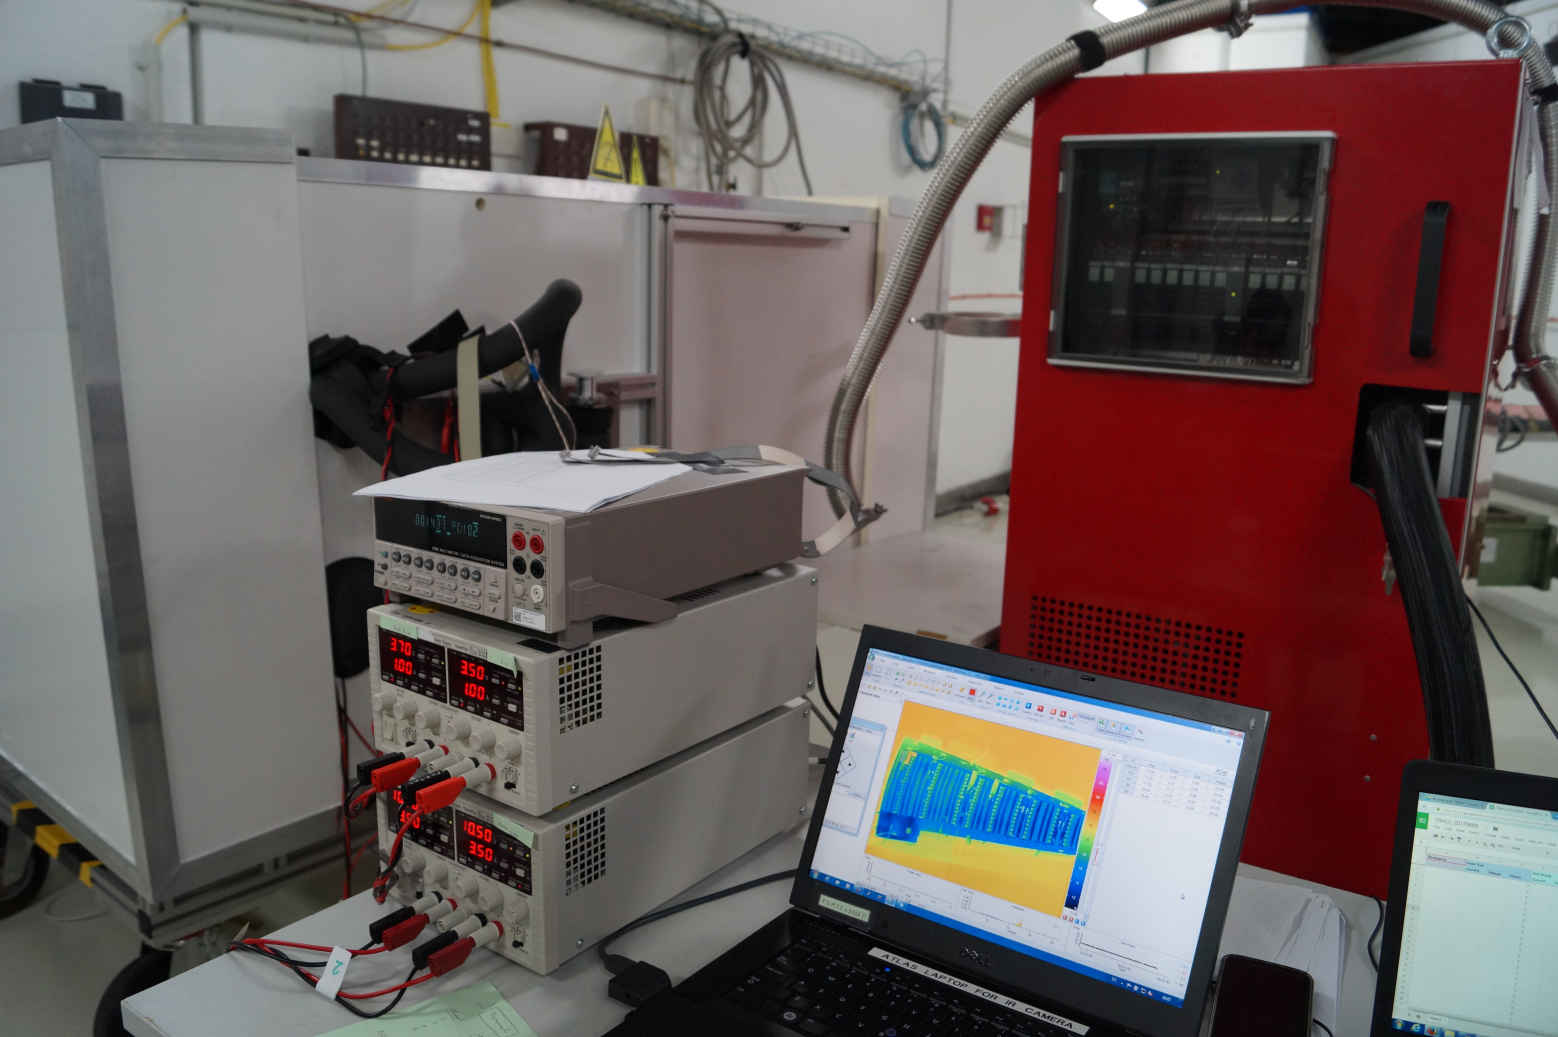
\includegraphics[scale=0.185]{Figures/Chapter02/ExperimentalSetup.jpg}
			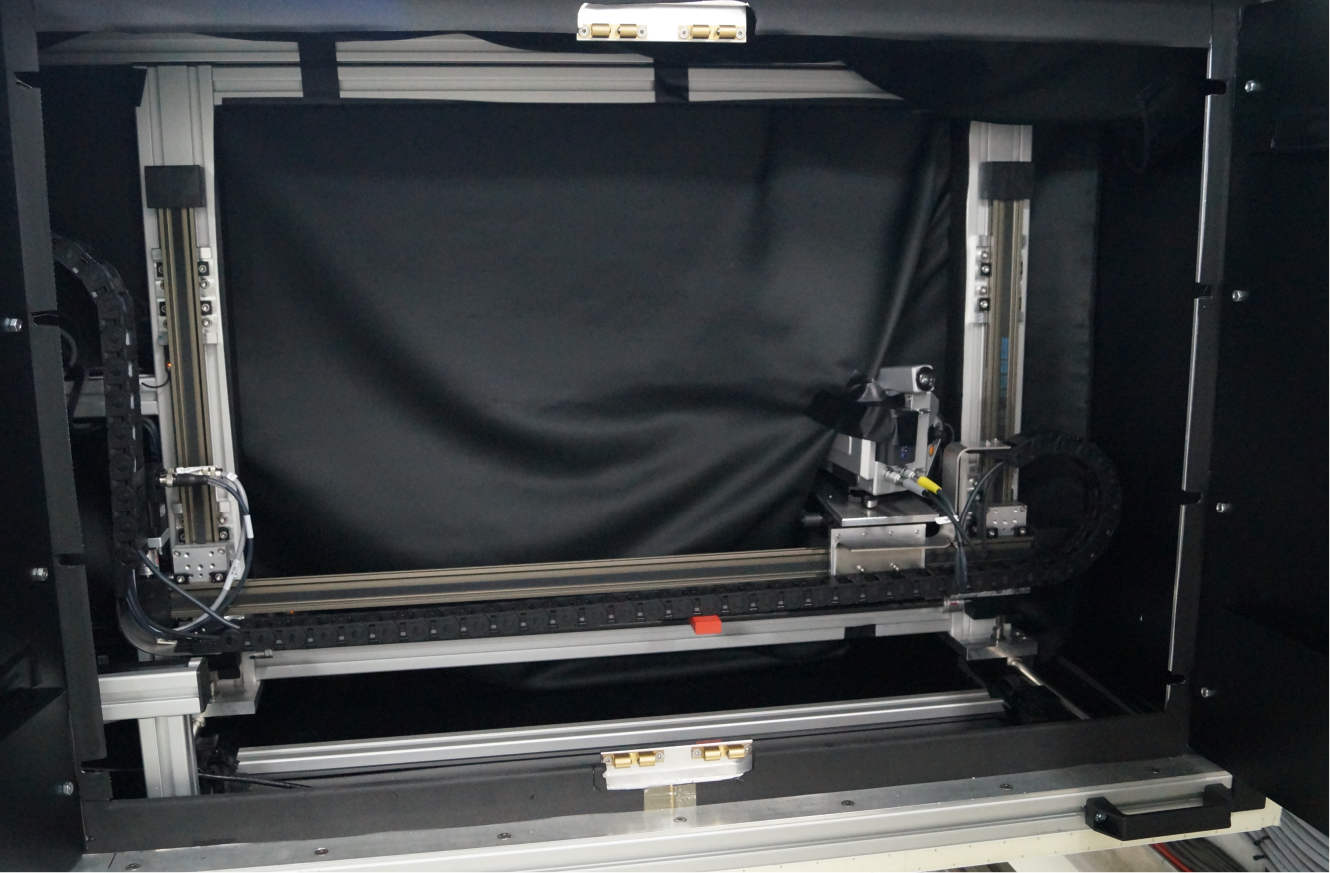
\includegraphics[scale=0.22]{Figures/Chapter02/BlackCurtine.jpg}
			\caption{Experimental setup used for the Petal’s thermal cycles. Right: a view of the chamber with new insulation, laptop for data acquisition, power supplies and Keithley (next to the laptop) and TRACI (Red box). Left: black curtain installation.}\label{fig2.7}
		\end{figure}
	
		This is particularly important for an accurate estimation of the apparent reflected temperature (See Section \ref{section3.1}). In addition, the DC-DC converters in modules R2 and R3 were covered with 3D-printed caps and black tape due to the fact that their heat created a “halo” of hot air (Figure \ref{fig2.8} right) around them that blurred the thermograms of that area of the Petal (Figure \ref{fig2.8} left).
		
		For cooling the Petal the \textit{Transportable Refrigeration Apparatus for CO$_{2}$ Investigation} (TRACI) Version 2 (100W) with Lewa pump was used (Figure \ref{fig2.7} left). This was the first time that a themo-mechanical petal prototype was cooled down using by-phase CO$_{2}$ in our set up. Previously, a water-glycol chiller was used, which greatly limited the lowest temperature that we were able to reach.
	
		\begin{figure}[ht!]
			\centering
			\captionsetup{justification=centering,margin=2cm}
			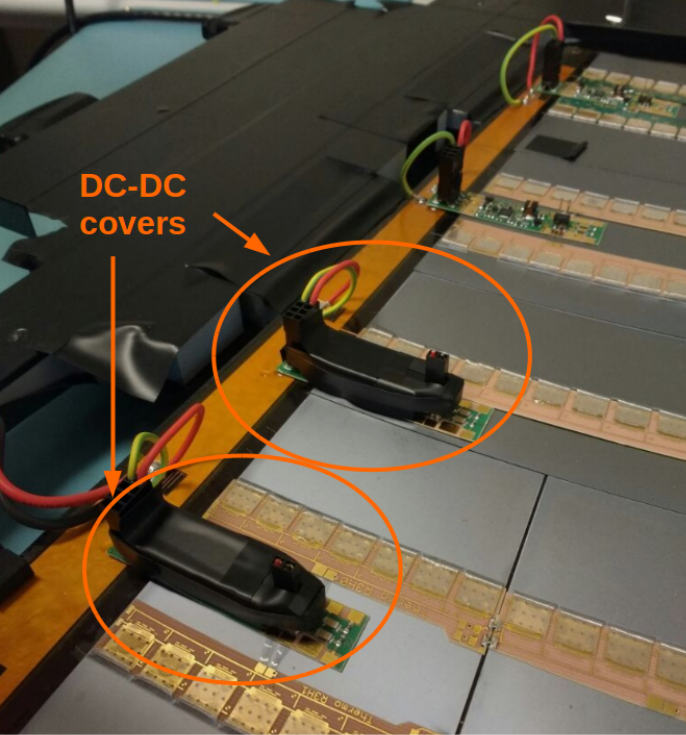
\includegraphics[scale=0.33]{Figures/Chapter02/DCDC_covers.jpg}
			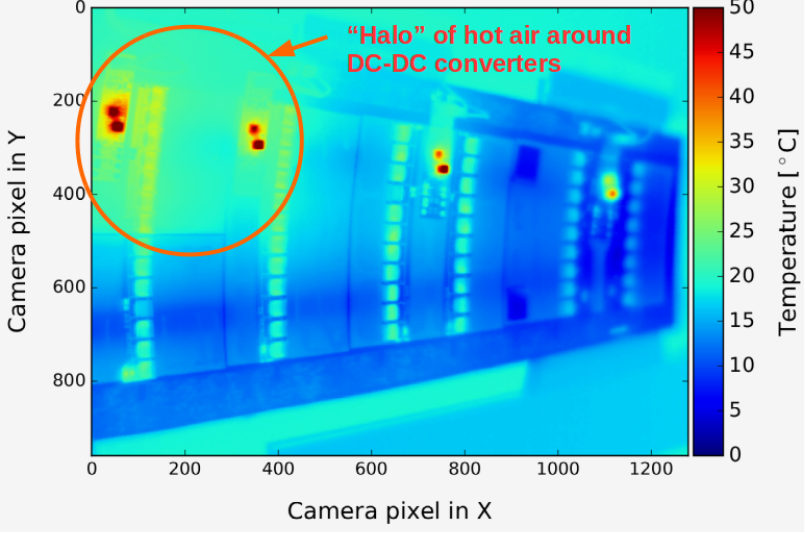
\includegraphics[scale=0.46]{Figures/Chapter02/HaloThermogram.jpg}
			\caption{Unpolished side of the Petal showing the DC-DC covers (left) and the thermogram where that “halo” of hot air around them is visible inside the circle (right).}\label{fig2.8}
		\end{figure}
	
		By controlling the CO$_{2}$ pressure in the experiment we were able to adjust the desired temperature working point. Using this method temperatures of near -25\space$^{\circ}$C were reached.
		
		The petal is equipped with 9 dummy circuits simulating the heat emitted by the readout electronics (6 module electronics + 1 EoS) per side. An important aspect for the prototype operation is that the powerboards should have a constant power consumption of $\sim$25W and the EoS $\sim$3W in each side of the petal. To power each side's powerboards and both EoS two TTICPX400 power supply units were used. The modules voltage is set to 10.5V and the current to 2.5A. In the case of the EoS the current is set to 1.0A (for both sides) and the voltage to 3V. However, as the resistance of the circuit changes with temperature we had to vary the voltage accordingly to keep the 3W of power consumption constant. For cycle 2 we did it manually but for cycle 9, as part of the Summer Student program, the student involved in the IR project was able to automatize the process by creating a program that automatically varied the voltage input to keep a steady 3W power consumption \ref{ref10}.
		
		In addition, a Keithley 2700 multimeter was used to register the readings from additional PT100 thermocouples using 4 wire sensing and some other important TRACI parameters like, for example, CO$_{2}$ flow, CO$_{2}$ temperature before experiment (petal), CO$_{2}$ temperature after experiment, pressure setpoint and pressure of the CO$_{2}$ in the experiment.
		
		The additional thermocouples were placed as follows (for cycle 2): 2 on the inlet/outlet pipes (glued), 2 in R3 module silicon surface (maintained by a piece of high emissivity black tape): 1 between the ASICs and 1 in the corner next to R4 (Figure \ref{fig2.9} top). For cycle 9 four extra thermocouples were placed in R0, R1, R4 and R5 as shown in Figure \ref{fig2.9} (bottom).
		
		\begin{figure}[H]
			\centering
			\captionsetup{justification=centering,margin=2cm}
			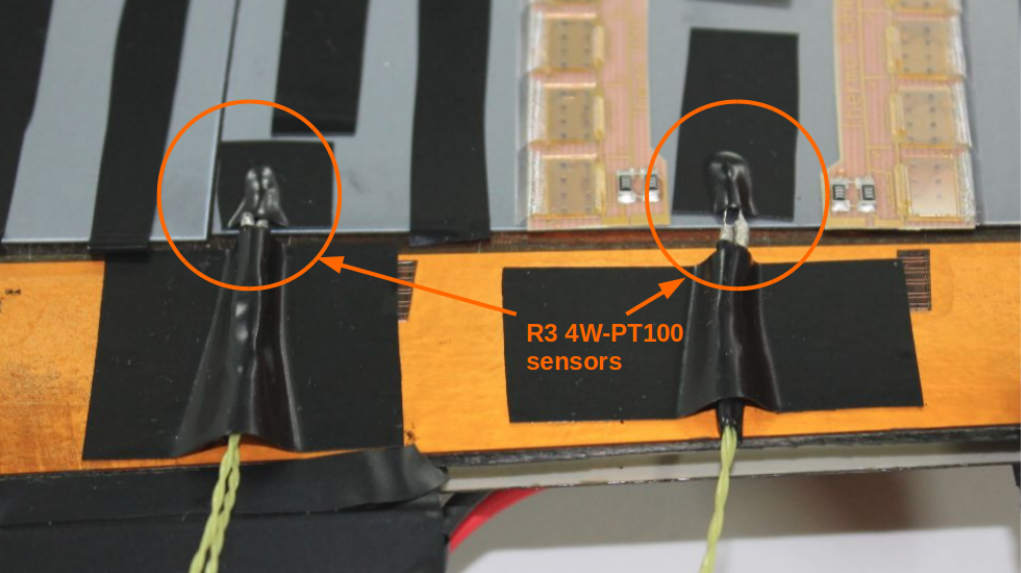
\includegraphics[scale=0.47]{Figures/Chapter02/R3PT100CloseUp.jpg}
			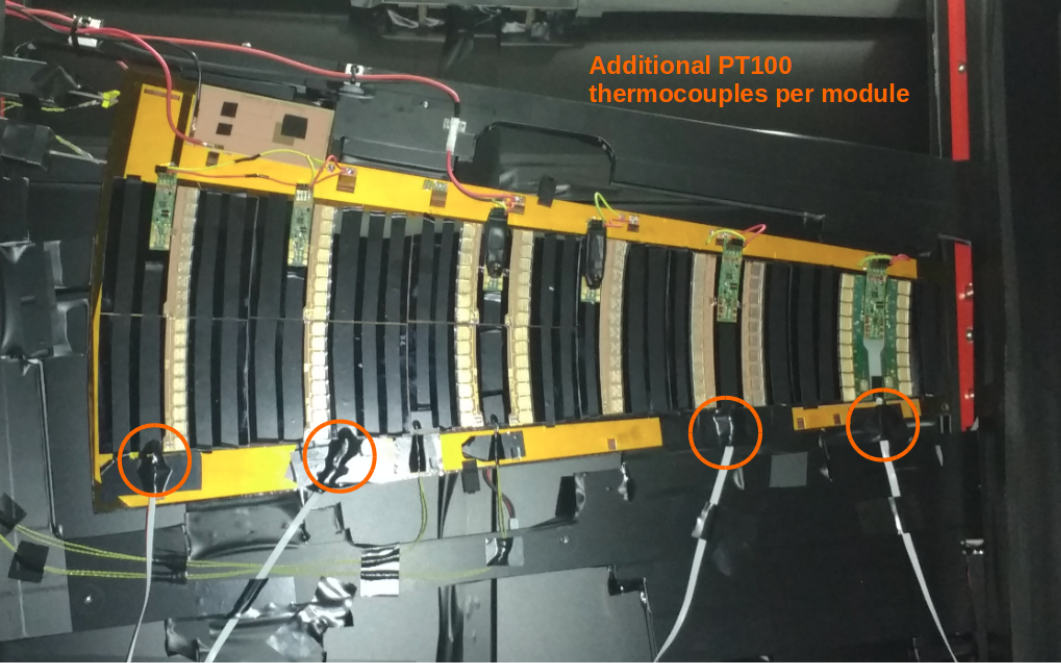
\includegraphics[scale=0.45]{Figures/Chapter02/AdditionalPT100perModule.jpg}
			\caption{Close-up of the unpolished side of the Petal showing the 2 PT100 thermocouples attached to R3 module (top). Polished side of the Petal ready for the thermal test. The additional PT100 thermocouples placed at each module (except R2) are visible (bottom).}\label{fig2.9}
		\end{figure}

	\clearpage
	
	% % % Set the style for this file:
\pagestyle{standard}

% % % Beginning of the chapter
\chapter{Preliminary measurements.}\label{chapter3}

	% % % Set the style for the first page:
	\thispagestyle{chapter-first-page}

	\section{Apparent reflected temperature estimation.}\label{section3.1}
	
		In order to correctly estimate the emissivity of any surface, it is very important to determine first the surface apparent reflected temperature. This is crucial, especially for low emissivity materials where a significant contribution is in fact due to the reflected radiation.
		
		A simple method can be used to determine the apparent reflected temperature. To do it, a low emissivity material is needed, usually, an aluminum foil or any other aluminum surface. This method is described as follows:
		
		\begin{enumerate}[label={\arabic*)}]
			\item Place a piece of crumpled and re-flattened aluminium foil in the same position of the object to be measured.
			\item Set the IR camera emissivity internal control to 1.00 and the distance to 0 m.
			\item Point the IR camera to the target (aluminum surface) and select a region of interest (ROI).
			\item Read the value from IR camera on the ROI.
			\item Take the measured value as the apparent reflected temperature.
		\end{enumerate}
	
		Aluminum foil has very low emissivity ($\sim$0.04) and therefore we are certain that almost all IR radiation coming from its surface is reflected from other sources. The camera emissivity is set to 1.00 and the distance to 0 so that the IR camera software does not apply any further correction. The crumpling is done to allow reflections from several directions. For this reason the ROI selected should be as wide as possible since this effect must be averaged out to obtain an accurate estimate of the apparent reflected temperature.\bigskip
	
	\section{Influence of the angular distribution of the emitted IR radiation.}\label{section3.2}
	
		In order to determine whether the viewing angle of the camera with respect to the normal of the petal's surface is a determining factor in our analysis, an study of the angular dependence of emissive power was performed using an aluminum rod filled with hot water placed in the same position as the petal. Using a strip of high emissivity black tape along the rod’s frontal face we were able to measure the variations in temperature due to the viewing angle (Figure \ref{fig3.1}).
	
		\begin{figure}[ht!]
			\centering
			\captionsetup{justification=centering,margin=2cm}
			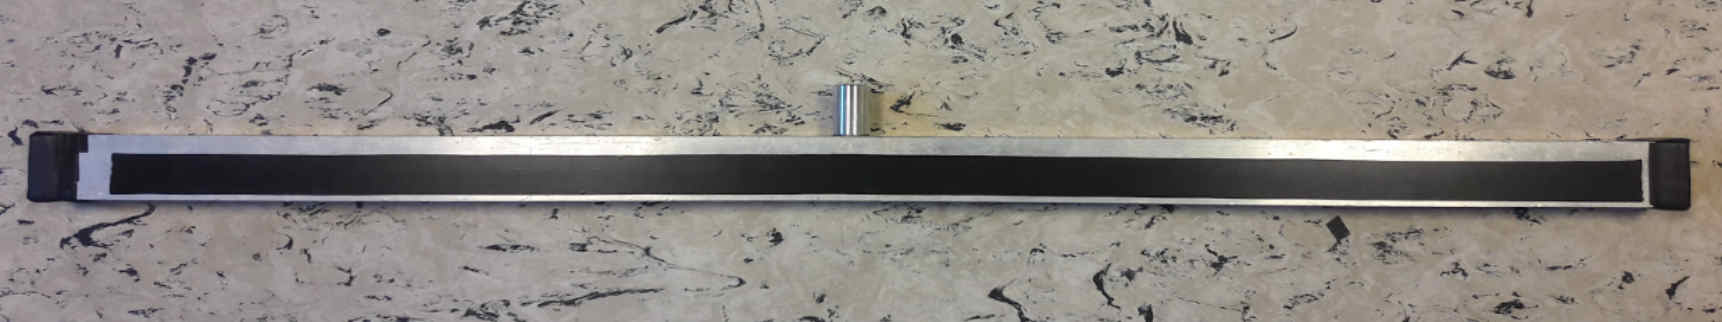
\includegraphics[scale=0.30]{Figures/Chapter03/AluminumRod.jpg}
			\caption{Aluminum rod used to study the angular dependence of emissivity}\label{fig3.1}
		\end{figure}		
	
		A set of measuring areas (ROIs) was defined along the rod using the IR camera software (IRBIS) and a thermocouple was inserted inside the rod in direct contact with the water in order to be able to determine the real temperature of the rod surface. The results can be seen in Figure \ref{fig3.2}. 
		
		We observed that the temperature variations along the rod are within 1$^{\circ}$C, including the error bands, from an angle of 0$^\circ$ (with respect to the normal of the rod’s surface) to roughly 30$^\circ$. For the central values this difference is less than 0.2$^{\circ}$C. This is a relatively small variation for that angular range and even though we see a drop in the markers temperature with respect to the real temperature of 34.6$^{\circ}$C (measured with a thermocouple directly inside the rod) the error magnitude make us conclude that, within this uncertainty, the angle influence on the IR temperature measurements is quite negligible.
		
		\begin{figure}[ht!]
			\centering
			\captionsetup{justification=centering,margin=0cm}
			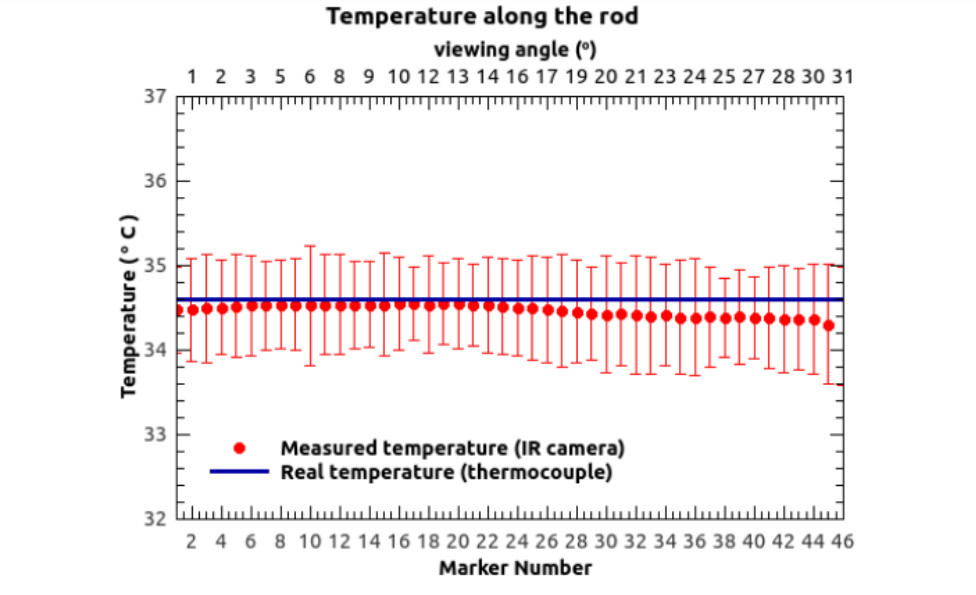
\includegraphics[scale=0.5]{Figures/Chapter03/RodAngularTempResults.jpg}
			\caption{Angle study results using the aluminum rod filled with water at 34.6$^{\circ}$C. The marker positions do not cover the entire rod since it is larger than the petal and some portions fall out of the viewing field of the camera.}\label{fig3.2}
		\end{figure}\bigskip
	
	\section{IR camera spectral response.}\label{section3.3}
	
		From Equation \ref{eq1.16} it can be seen that if we can accurately estimate the emissivity, the apparent reflected temperature and the IR camera spectral response function ($R$) we should be able then to obtain the real temperature of the object for any given spectral power value reported by the camera ($N_{meas}$). 
		
		In order to estimate the $R$ factor we can simply take the emissive power measurements of a surface of known emissivity, the real temperature and the apparent reflected temperature and then use the same Equation \ref{eq1.16} to derive the $R$ scale factor. As this factor only depends on the IR camera, it can be used later on in the analysis as long as we don’t use a different camera.
		For obtaining the scale factor we used an aluminum bucket, which we filled with hot water and recorded the IR power density on several points of the surface (always at the same depth). The measured aluminum surface was coated with high emissivity black\footnote{{\footnotesize Note that the "visible" color of the tape has nothing to do with the emissivity value. It could have been a red, green or even white. The color of the tape is a property related with the visible wavelengths in electromagnetic spectrum while the infrared properties are related with the IR part of the spectrum.}} tape as the water temperature went down to test the temperature dependence of the results (Figure \ref{fig3.3}).
		
		\begin{figure}[ht!]
			\centering
			\captionsetup{justification=centering,margin=2cm}
			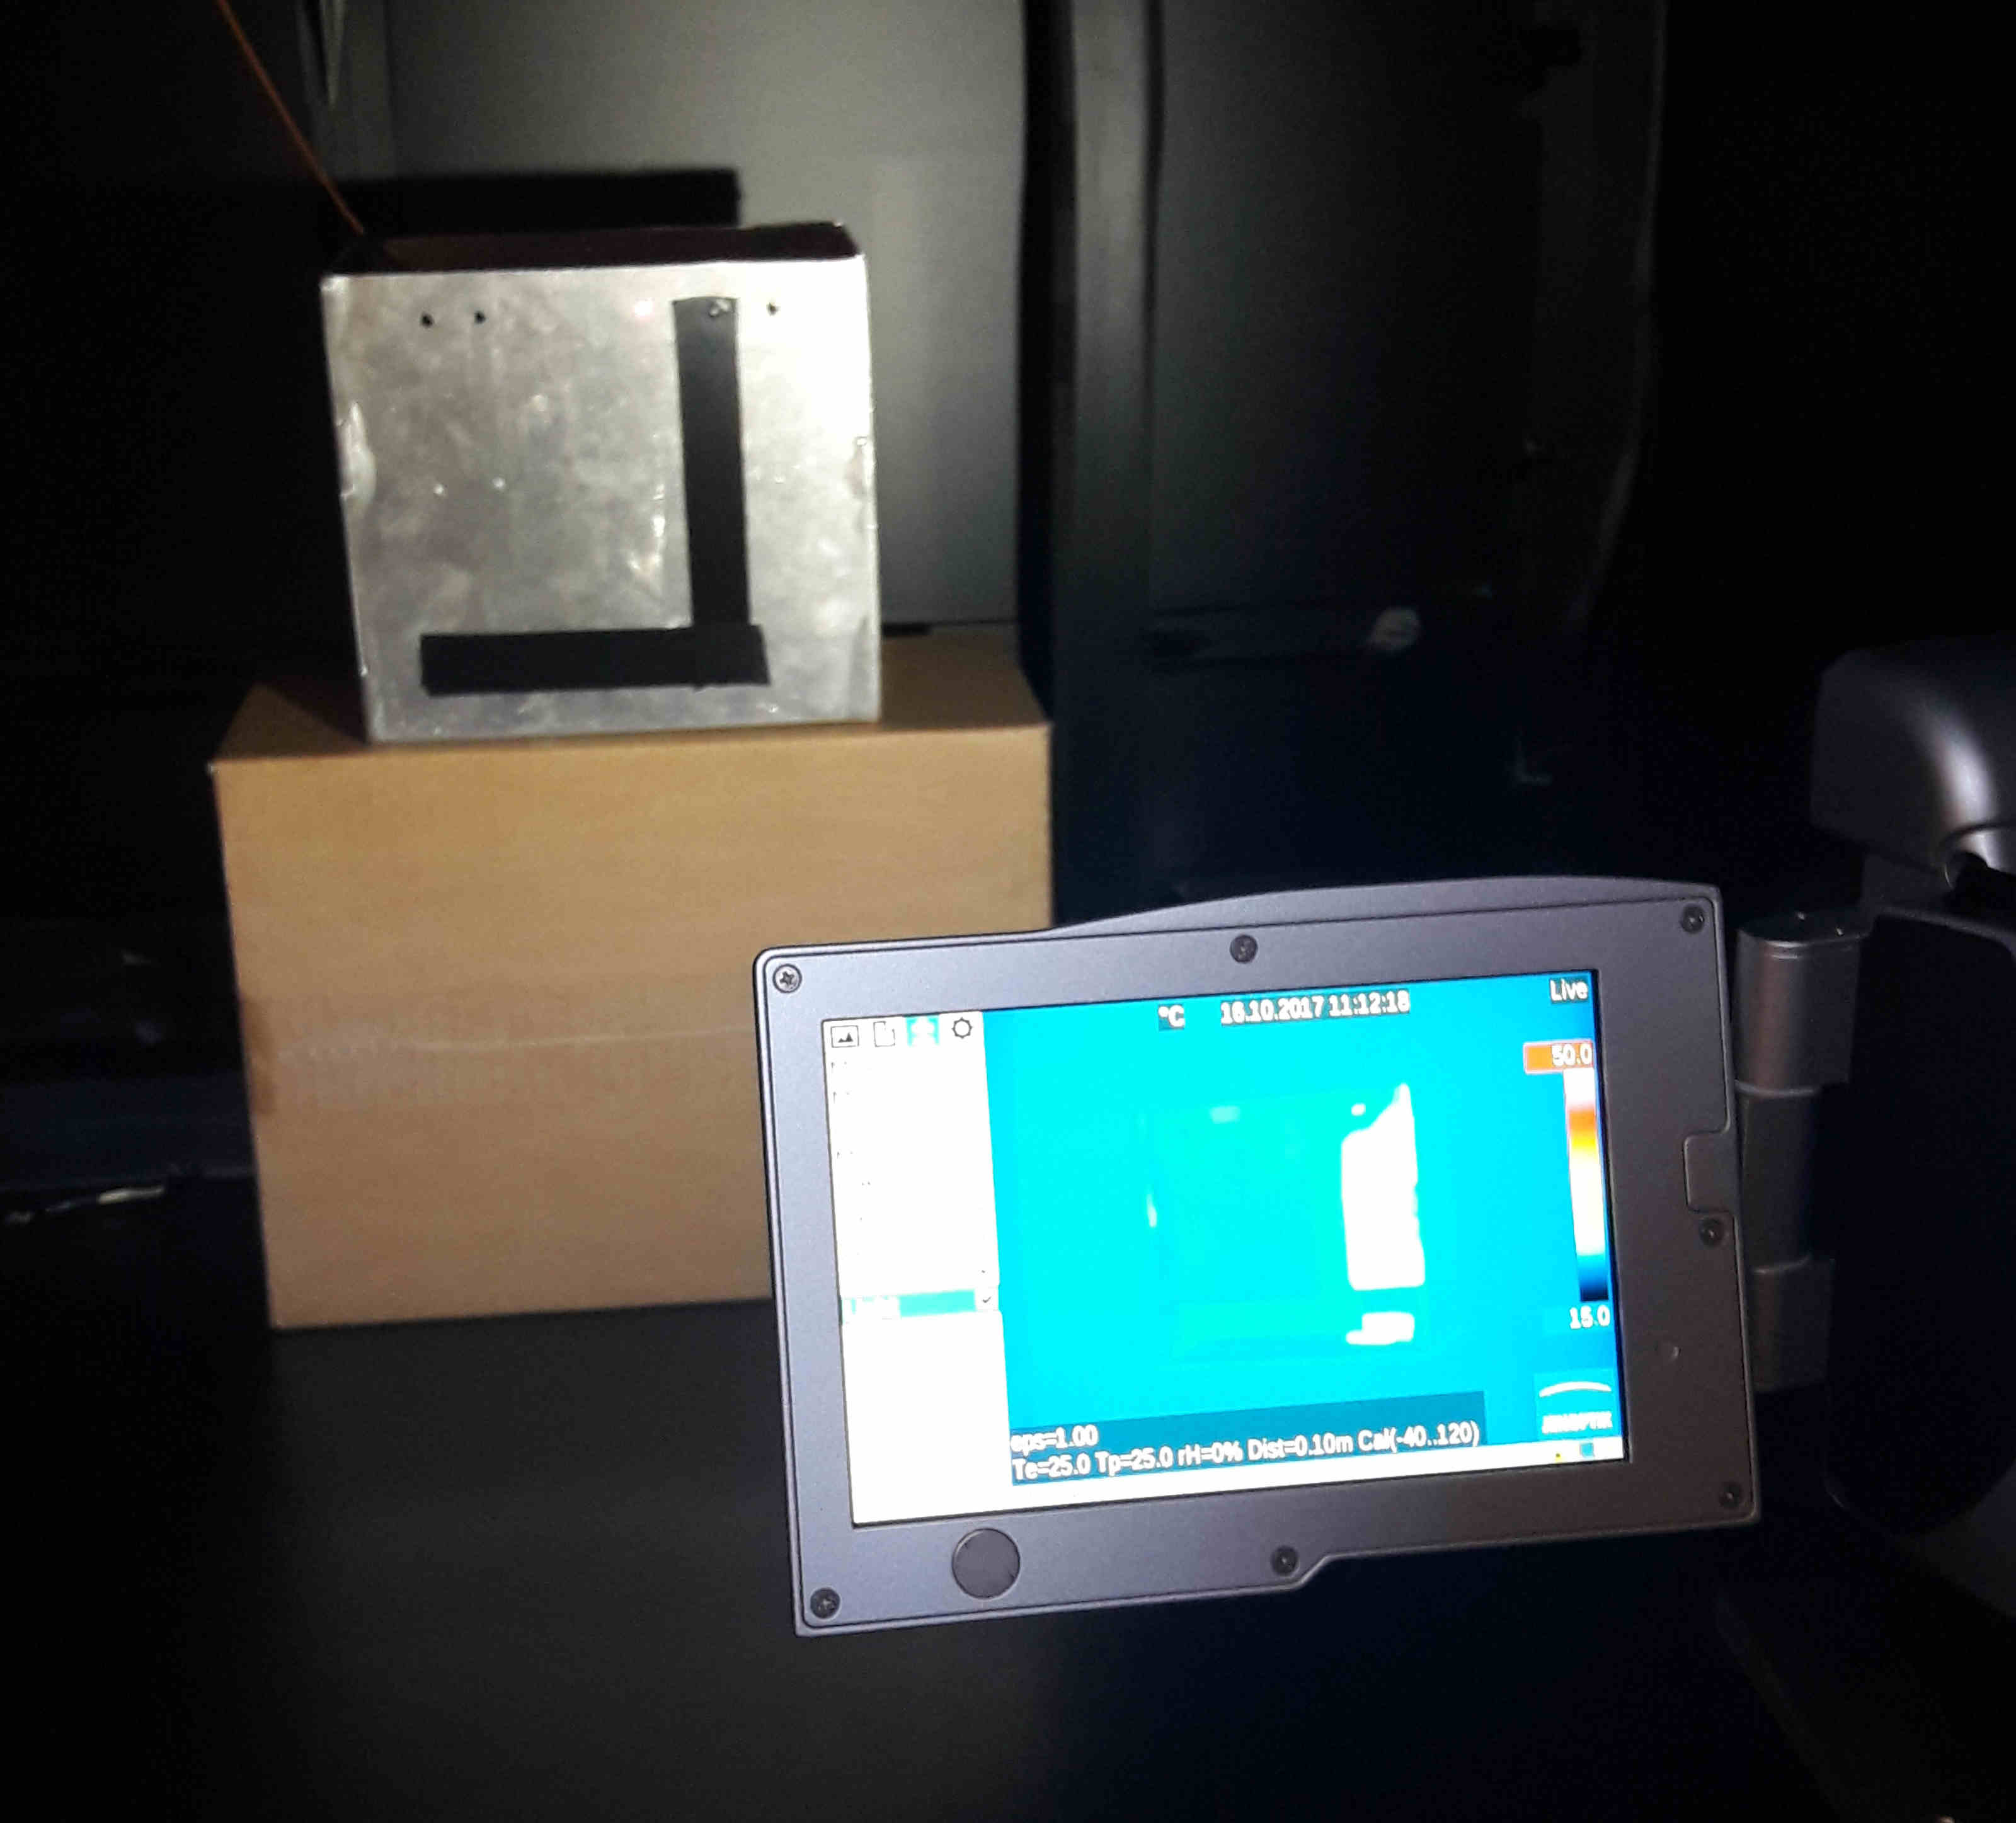
\includegraphics[scale=0.1]{Figures/Chapter03/CameraAndBucket.jpg}
			\caption{Experimental setup to calculate the IR camera spectral response function. Measurements were performed placing measurement markers along the horizontal black tape in the camera IRBIS software.}\label{fig3.3}
		\end{figure}
		
		With this scale factor and Equation \ref{eq1.16} we could estimate the emissivity at pixel level if we had a thermogram in which the real temperature of all the pixels is known. That would allow correct the thermograms in emissivity without the need of covering the Silicon surfaces with high emissivity materials (See Section \ref{section4.1}). That is the so called “baseline image” correction method.
	
		Figure \ref{fig3.4} (left) shows the results of the estimation of the $R$ scale factor for the IR camera using the aluminum bucket filled with hot water. Furthermore, to test the validity of the method we used as well a petal thermogram of which we knew the real surface temperatures, that is, the petal at room temperature without cooling nor electronics powered on. Figure \ref{fig3.4} (right) shows the scale factor estimation on the petal.
		
		\begin{figure}[H]
			\centering
			\captionsetup{justification=centering,margin=2cm}
			\includegraphics[scale=0.5]{Figures/Chapter03/BucketScaleFactors.pdf}
			\includegraphics[scale=0.5]{Figures/Chapter03/PetalScaleFactors.pdf}
			\caption{Fits of the IR camera response scale factor calculated for different temperatures using the aluminum bucket (left) and using a petal thermogram (right).}\label{fig3.4}
		\end{figure}
		
		For the calculations, the values of the black tape in silicon modules R0, R1 and R2 were used, showing consistent results with the values obtained with the aluminum bucket. The uncertainty shown is the fit’s root mean squared error. With this test we corroborated that this factor is only dependent on the IR sensor/camera and independent of the temperature and the surface.\bigskip
		
		
		

	
	\clearpage
	
	% % % Set the style for this file:
\pagestyle{standard}

% % % Beginning of the chapter
\chapter{Results and discussion}\label{chapter4}

	% % % Set the style for the first page:
	\thispagestyle{chapter-first-page}

	\section{Petal thermal cycles.}\label{section4.1}
	
		For both thermal cycles the set points were selected by varying the CO$_{2}$ pressure in such a way that we go from room temperature to the lowest possible temperature and back to room temperature in steps of 5\space$^{\circ}$C. Then, at each set point, the following data is recorded:
	
		\begin{enumerate}[label={\arabic*)}]
			\item Inlet/outlet pipes temperatures (PT100).
			\item Temperature readings (PT100) on the silicon surface at each module (See Figure \ref{fig2.9}).
			\item CO$_{2}$ flow.
			\item Temperature of the CO$_{2}$ going in/out of the petal.
			\item Pressure of the CO$_{2}$ going into the petal and the difference to the pressure setpoint.
			\item Ambient temperature and RH inside the chamber.
			\item Voltage/current readings from the power supply units.
		\end{enumerate}
	
		Also, the Petal thermograms are recorded following the method described in Section \ref{section2.3} at each step. The results are shown in Figure \ref{fig4.1} for both cycles 2 and 9. Uncertainties of the IR measurements have not been included not to overload the plots but, as discussed also in Section \ref{section2.3}, the main source of uncertainty comes from the IR camera itself. 
	
		\begin{figure}[ht!]
			\centering
			\captionsetup{justification=centering,margin=0cm}
			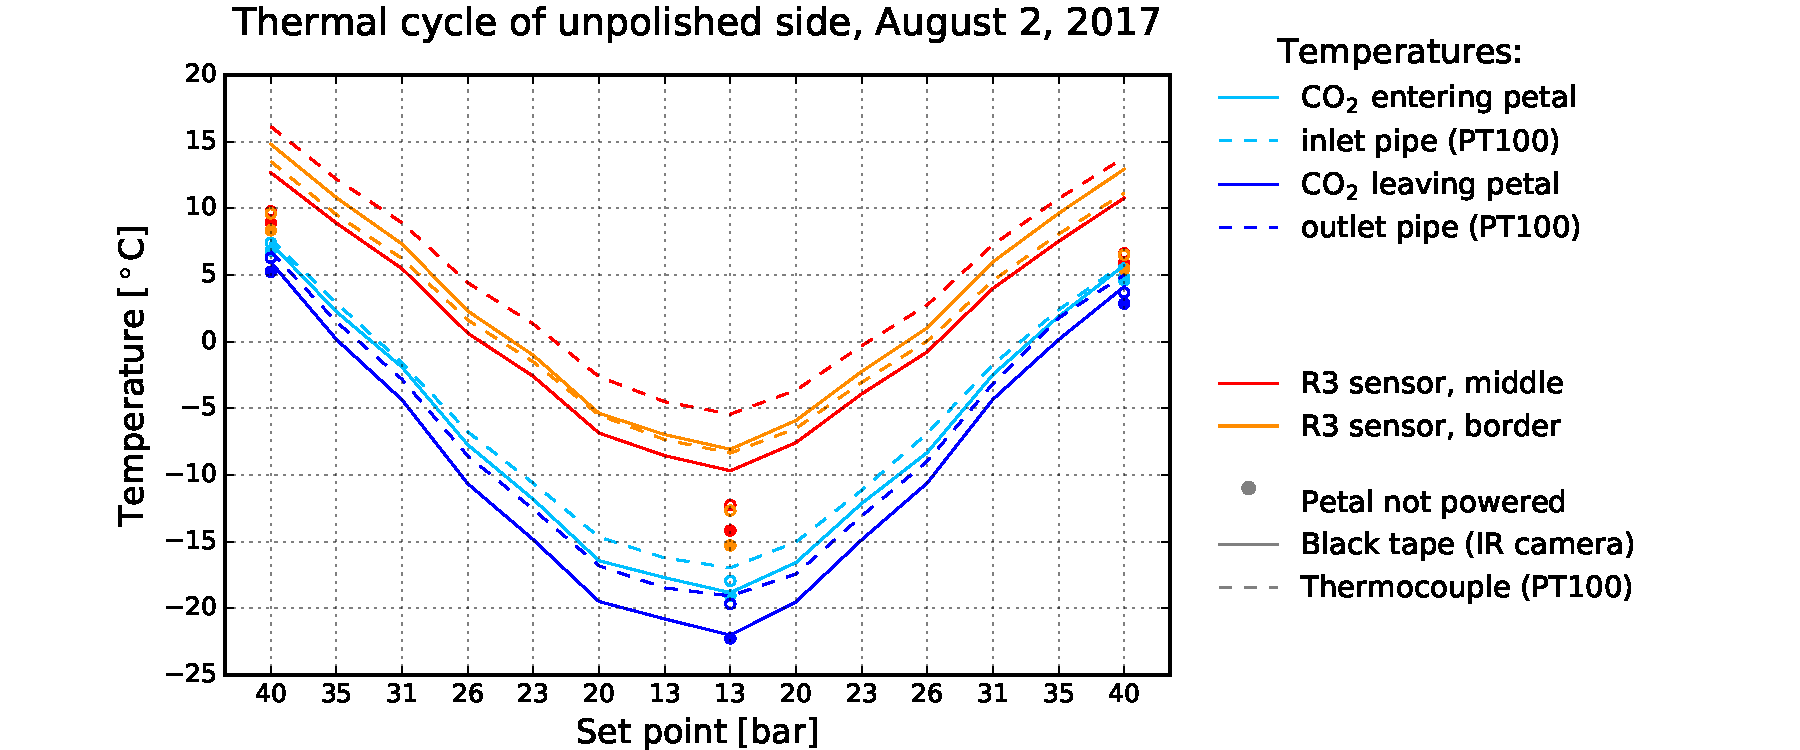
\includegraphics[scale=0.45]{Figures/Chapter04/unwrapped_cycle_2_201711121522.pdf}
			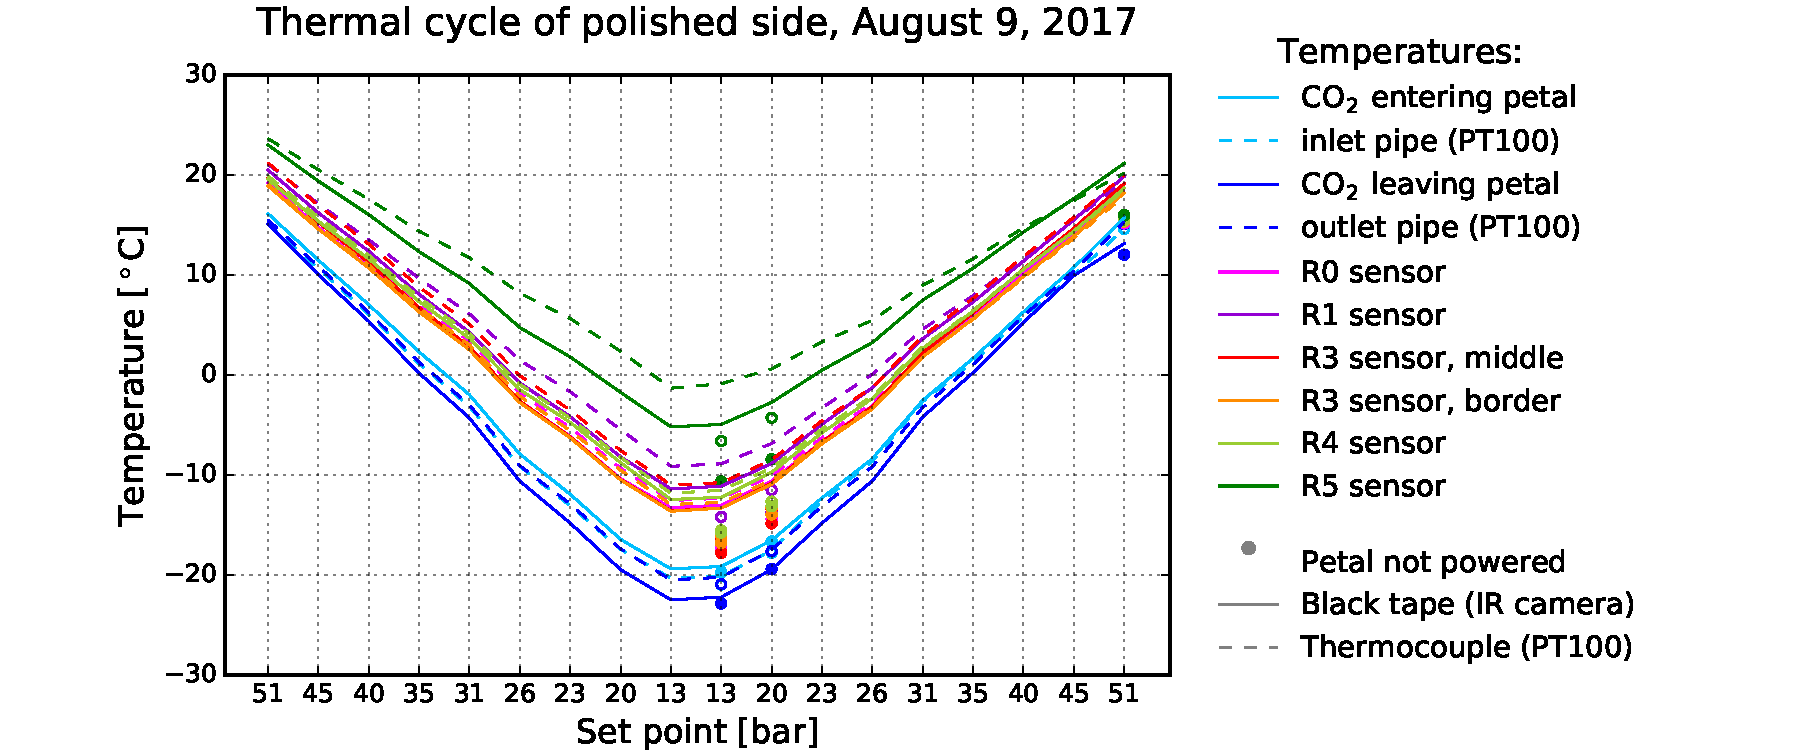
\includegraphics[scale=0.45]{Figures/Chapter04/unwrapped_cycle_9_201711121522.pdf}
			\caption{Temperature plots for the thermal cycles corresponding to the polished (front) and unpolished (back) sides. The dots represent set points with the Petal not powered and the lines correspond to set points with both sides of the petal powered. Solid lines and filled dots represent black tape readings with the IR camera (except CO$_{2}$ entering/leaving petal) and dashed lines and hollow dots represent thermocouple values.}\label{fig4.1}
		\end{figure}
	
		As it can be seen, with cycle 2 (cycle 9) we were able to reach temperatures of around -18\space$^{\circ}$C (-20\space$^{\circ}$C). For both cycles it is also notable that the returning CO$_{2}$ is colder, which is consistent with dual-phase cooling. We can also see that the PT100 thermocouple sensors report consistently higher temperatures that the TRACI sensors for both inlet and outlet pipes. Either we lost some cooling power due to thermal conductivity of the pipes, which is expected, or one of the sensors got incorrectly calibrated/placed. This situation is the opposite in cycle 9 with the inlet fluid temperature readings. In fact, for cycle 9, the inlet PT100 accidentally broke and had to be reglued which might explain the difference from one cycle to the other in the inlet pipe while the outlet remained somewhat the same. This indicates that a correct manipulation of the thermocouple sensors is crucial to obtain good reliability on the measurements.
		
		Another interesting test that we wanted to perform was the comparison between the temperature reported by the IR camera using the black tape method and the temperature measured with an alternative method on the same surface (e.g. using PT100 thermocouples). In order to perform such a test, the additional PT100 sensors placed on the silicon surface were hold in position using the same high emissivity black tape used for the strips of the “Zebra” Petal. For cycle 2 only two PT100s were used, as described in Section \ref{section2.4} while for cycle 9 four additional ones were placed. From Figure \ref{fig4.1} (top) we can see that the readings of the thermocouple and the IR camera are quite different for the sensor placed between the ASICs, possibly due to miss-contact with the silicon surface (the sensors had to be placed very carefully not to damage the silicon). The other PT100 sensor, on the other hand, shows relatively good agreement with the IR camera measurement. The situation in cycle 9 improved a bit more, in general, for the lowest setpoint, specially in the R0, R3(border) and R4, even though there are still large discrepancies (e.g. R5). With this results we also see that the tendency of the sensors is to not having memory (i.e. they are not damaged) after the thermal cycles, which was one of the main concerns that motivated the thermal tests.\bigskip
		
	\section{Comparison with FEA results.}\label{section4.2}	
	
		In order to compare the results with FEA simulations, the IR camera temperature measurements from ROI markers on the surface of the black tape strips was used. Figure \ref{fig4.2} (top two) shows the lowest point thermograms for cycles 2 and 9 where the tiny red squares are the IRBIS measurement markers. Using linear interpolation between the marker points corresponding to the black tape measurements we were able to produce an isotherm map of the sensors as shown in figure \ref{fig4.2}(bottom two). Figure \ref{fig4.3} shows the corresponding FEA simulation results \ref{ref15} for both cycle 2 (top) and cycle 9 (bottom).
		
		\begin{figure}[ht!]
			\centering
			\captionsetup{justification=centering,margin=2cm}
			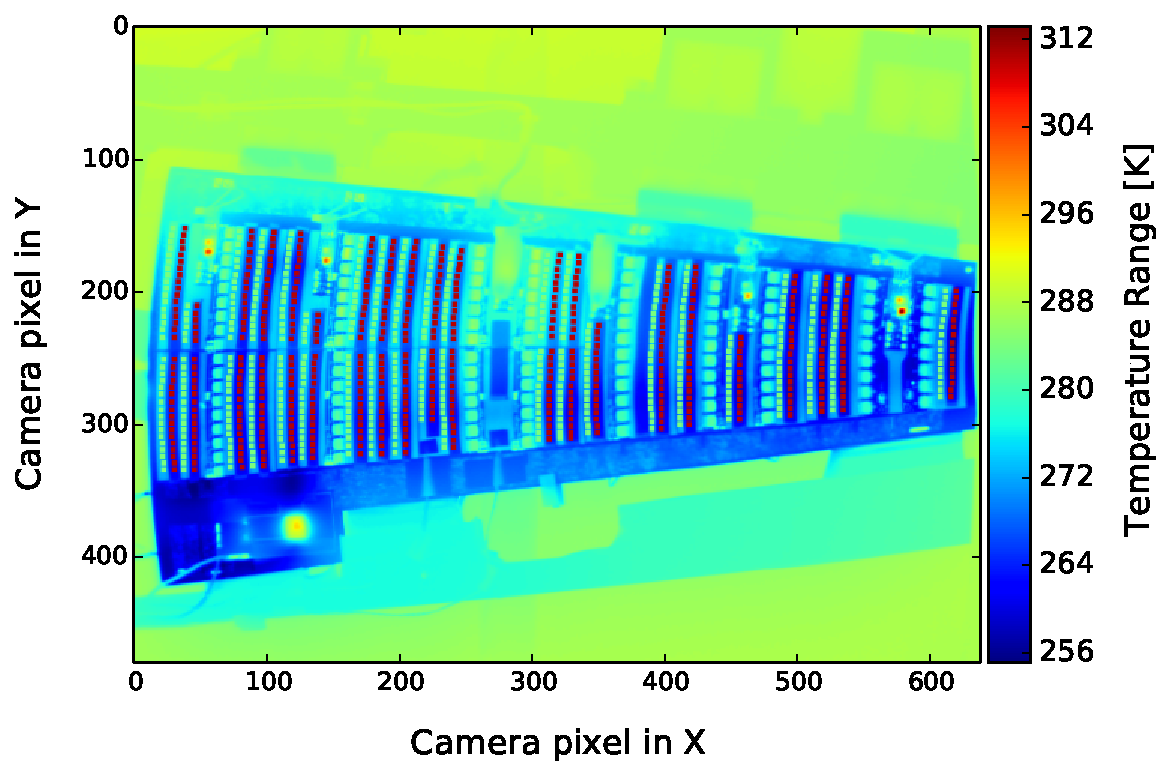
\includegraphics[scale=0.39]{Figures/Chapter04/thermo_Temp_20170803154926.pdf}
			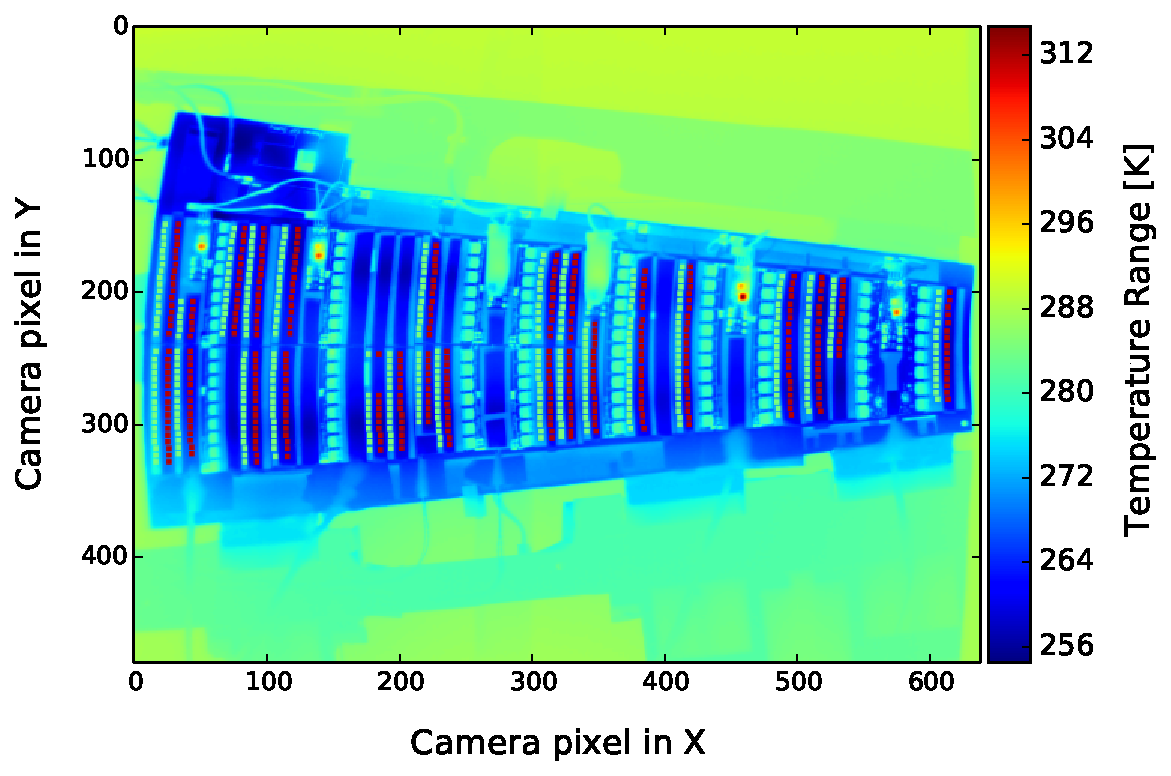
\includegraphics[scale=0.39]{Figures/Chapter04/thermo_Temp_201708101118_avg.pdf}
			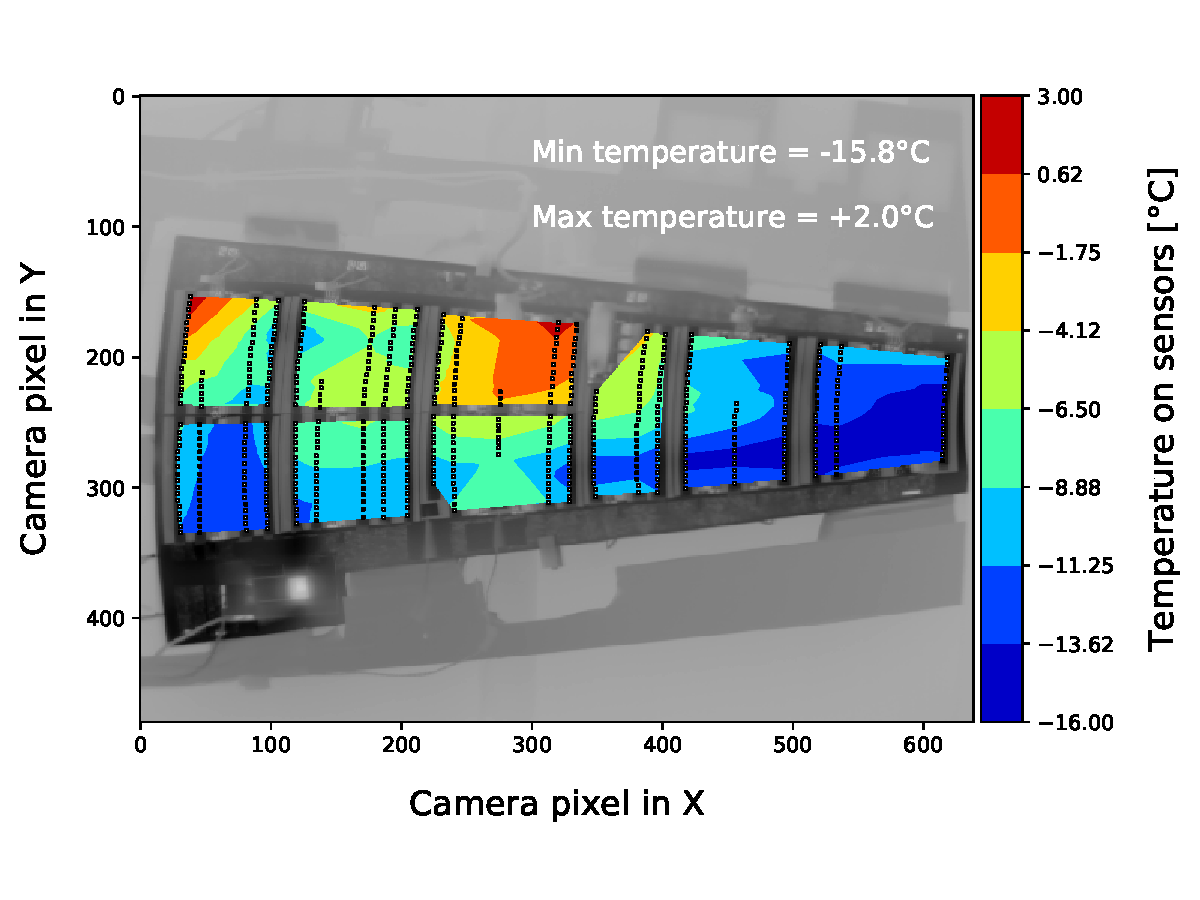
\includegraphics[scale=0.39]{Figures/Chapter04/thermogram_markers_2_201711271001.pdf}
			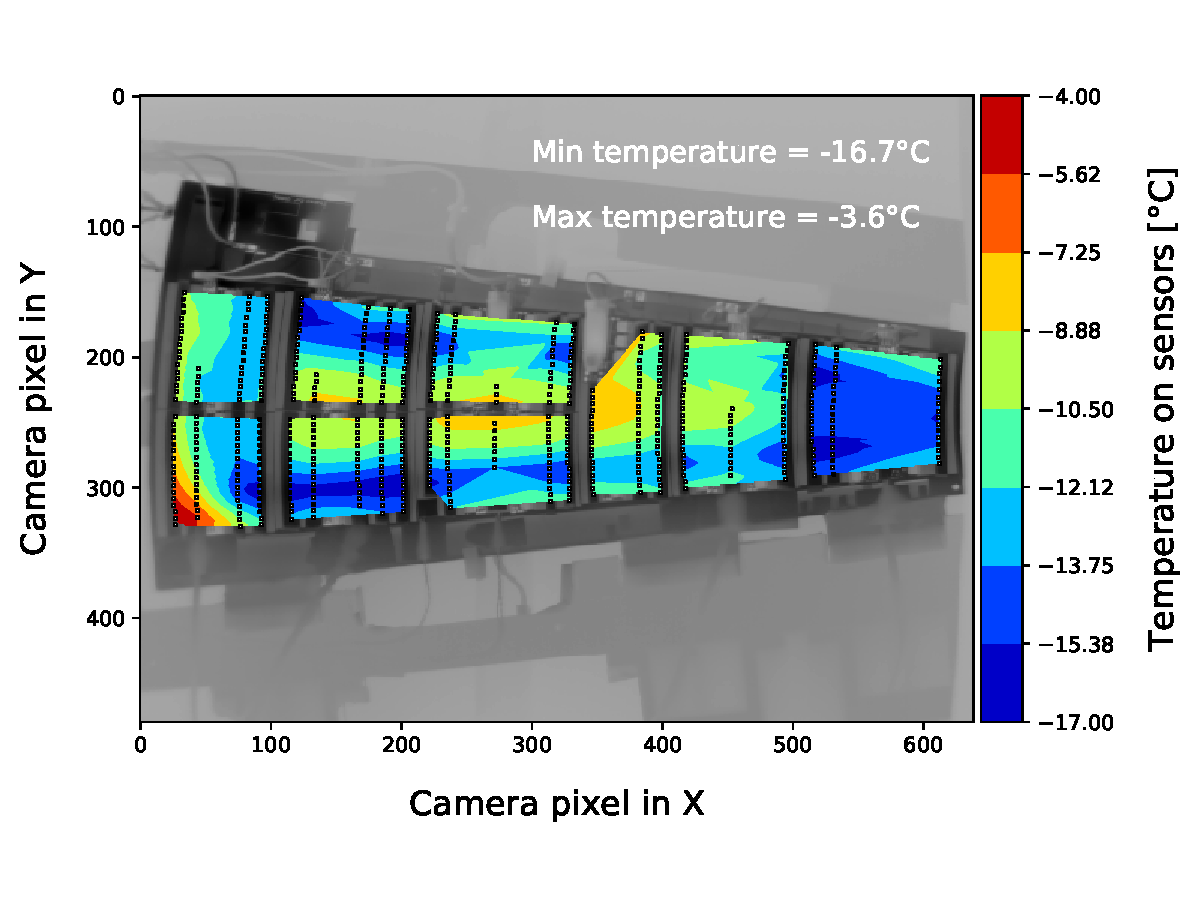
\includegraphics[scale=0.39]{Figures/Chapter04/thermogram_markers_9_201711271006.pdf}
			\caption{Thermogram of the lowest setpoint in cycle 2 (top left) and cycle 9 (top right) showing the IRBIS measurement areas (markers) defined on the black tape (red squares) and the corresponding silicon surface ones (blue squares). The linear interpolation isotherms for the sensors are shown in the two bottom images.}\label{fig4.2}
		\end{figure}
		
		Before discussing the differences between the images in Figure \ref{fig4.3}, we must say that this is to some extent an unfair comparison. While in FEA one have access to virtually every temperature point we are limited here by the number of markers and their uncertainty. Furthermore, the characteristics of the FEA model are not exactly compatible (e.g. power board thickness, cooling loop) and the very complicated convection/absorption with the air surrounding the Petal is very hard to model. In fact, we know that the values of temperature reported by the markers near the R3 electronics (hottest point) is greatly influenced by the “halo” surrounding it, as discussed in Section \ref{section2.4}. In addition, in that precise region of the image, the linear interpolation tries to figure out a large area where there is no experimental point and thus, this area should not be very well described.
		
		\begin{figure}[ht!]
			\centering
			\captionsetup{justification=centering,margin=0cm}
			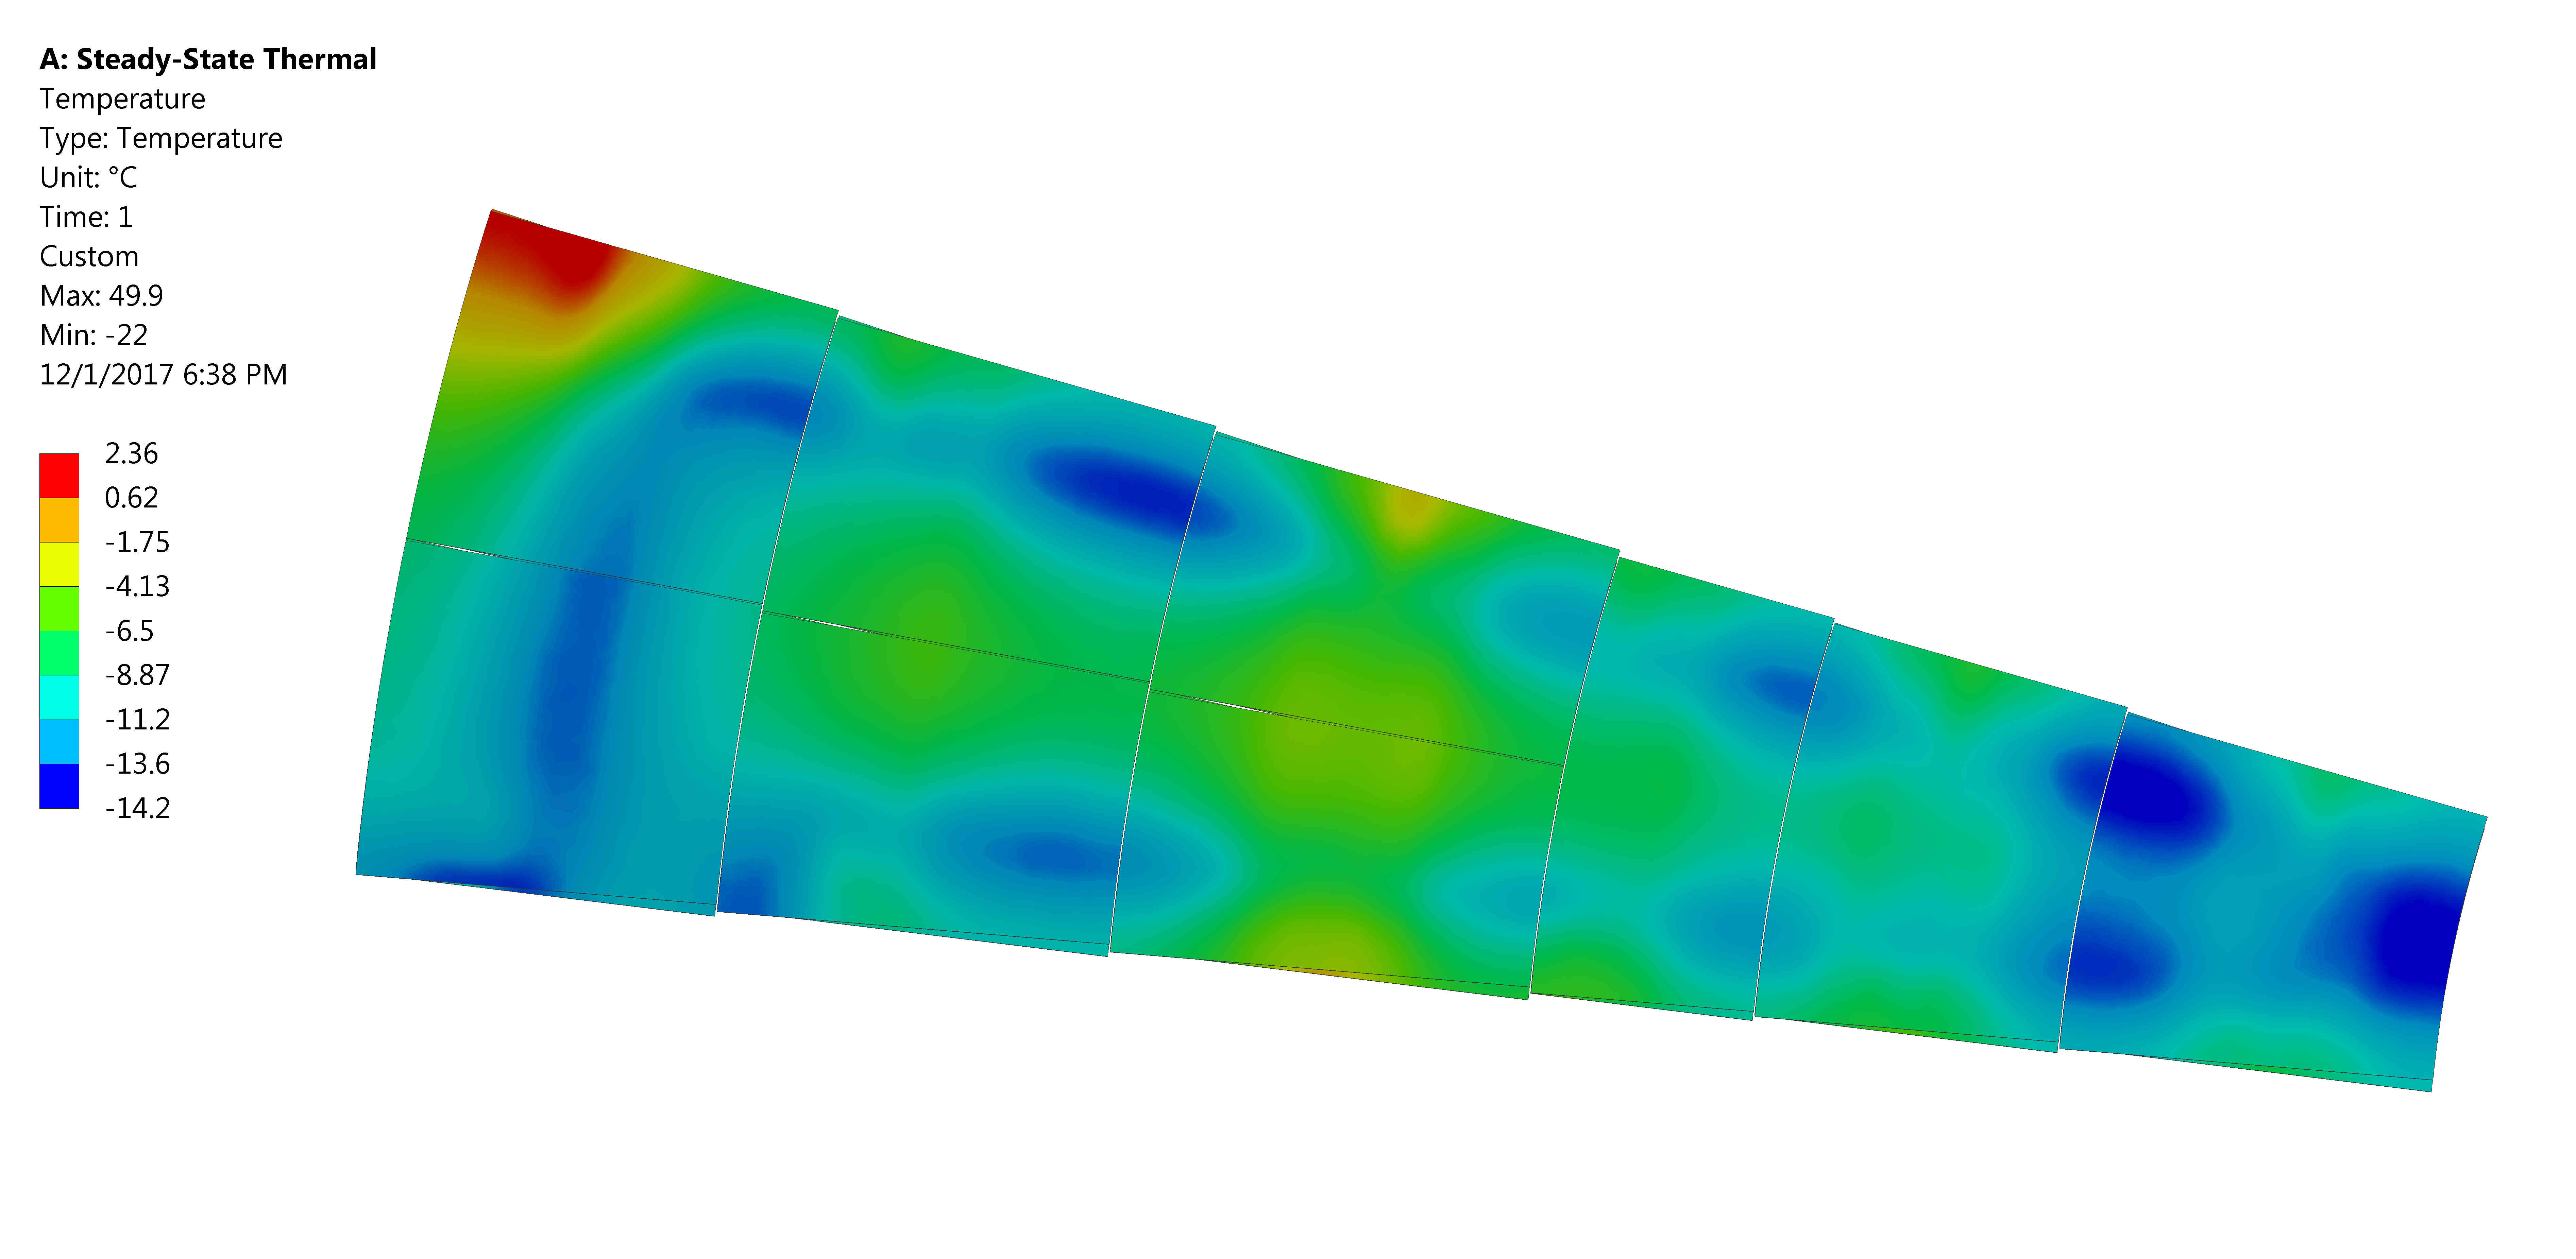
\includegraphics[scale=0.045]{Figures/Chapter04/FEA_thermogram_markers_2_201711271001.jpg}
			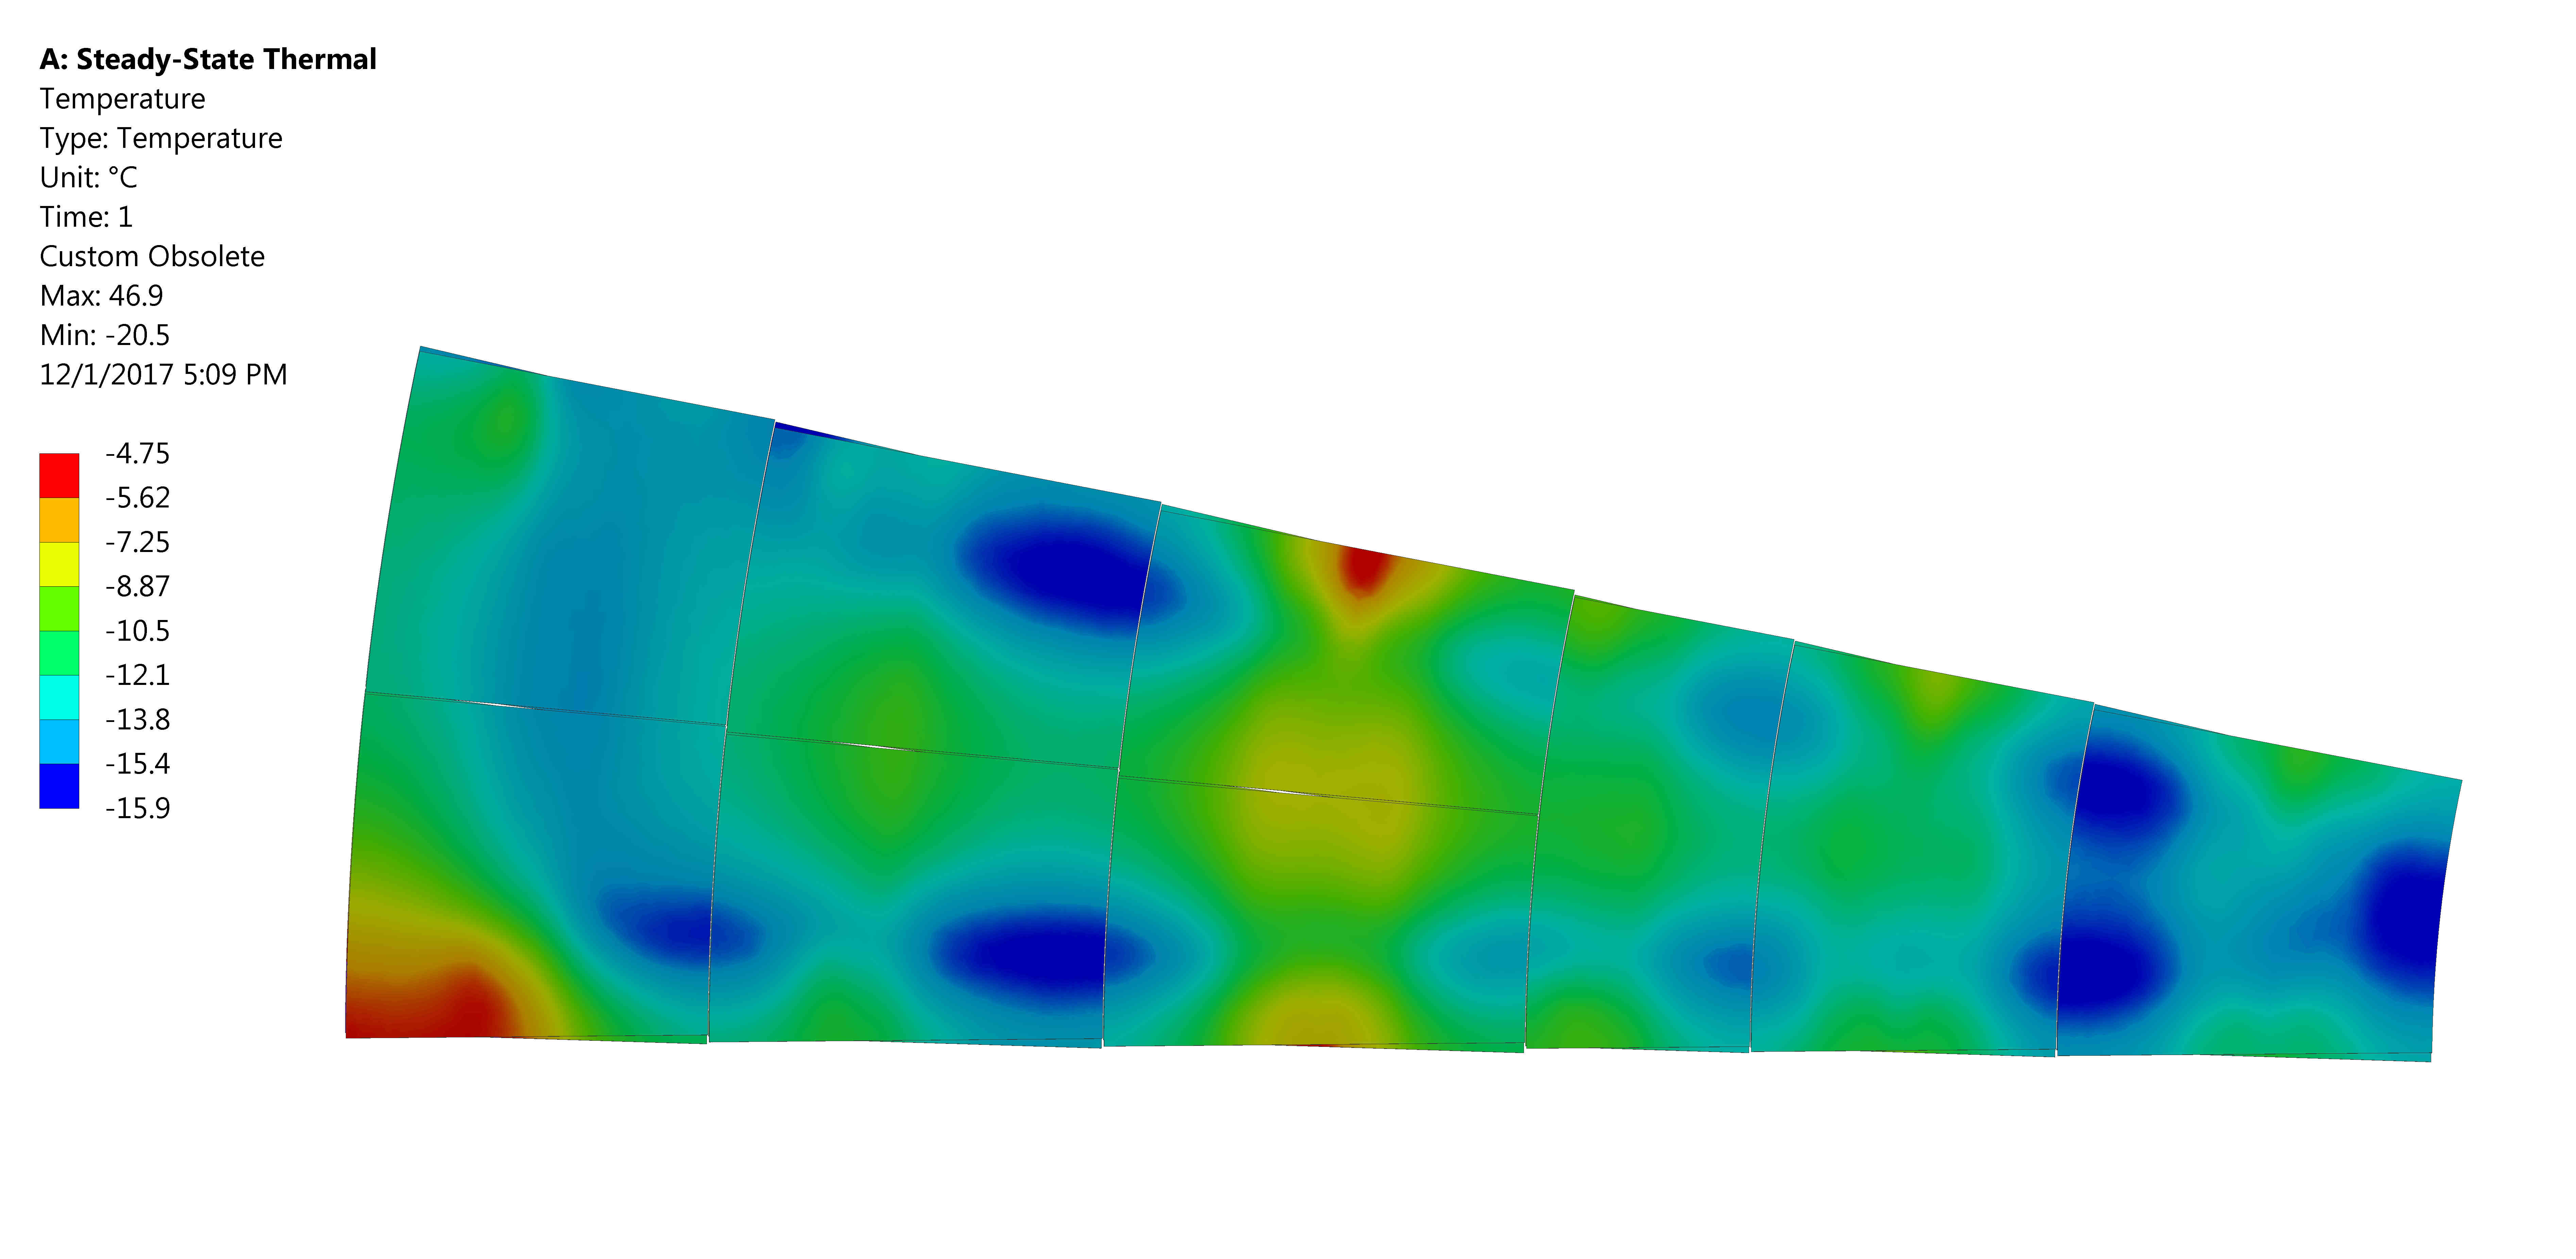
\includegraphics[scale=0.045]{Figures/Chapter04/FEA_thermogram_markers_9_201711271006.jpg}
			\caption{FEA simulations results for cycles 2 (top) and cycle 9 (bottom). The displayed temperatures correspond to the petal silicon sensors.}\label{fig4.3}
		\end{figure}	
		
		In general (without paying too much attention to the temperature magnitudes), some similar features can be found between the experimental results and the FEA model. For instance, the hot spot at the corner of R5 is well reproduced in the FEA model for both cycles. Additionally, the cold region corresponding to the path of the cooling pipe is quite similar. However, in places like R3 near the DC-DC converters, where the hottest point is expected to be, the agreement between IR measurements and simulations is worst due to the lack of experimental points in that area for a good linear interpolation.
	
	\section{Silicon emissivity estimation.}\label{section4.3}	
	
		As shown in the previous section, one of the factors affecting the robustness of the measurements is the lack of “resolution” by using the black tape method, even though more than 560 markers were created (by hand) on the surface of the silicon sensors. This asks for more refined ways to measure the temperature of the silicon sensors. Furthermore, the black tape method is a quite invasive technique to use with the current prototype and for sure something to avoid during quality control with real Petals.
		
		A good first approach would be to try to estimate the silicon emissivity and then use this value to correct globally the IR image. As mentioned in Section \ref{section3.3}, a “relative” method using the black tape markers measurements as temperature reference can be used to calculate the emissivity of the silicon next to them employing Equation \ref{eq3.3}. The IRBIS software also has an emissivity calculator which reports the emissivity of a given pixel if we provide the real temperature of the pixel and the ambient temperature (apparent reflected temperature). However, as this variant is more like a black box to us, we decided to use both methods and compare the results. As mentioned also in Section \ref{section3.3}, Equation \ref{eq3.3} will only work for opaque surfaces (not transmissive) and for surface temperatures well away from the apparent reflected temperature. For those reasons we performed this study on the unpolished side of the Petal since the polished side is highly transmissive (Figure \ref{fig4.4}).
		
		Figure \ref{fig4.5} shows a profile plot of one of the black tape strips in sensor R3 at the lowest setpoint. We can see how both silicon and black tape markers readings show two minima corresponding to the position through which the cooling pipe goes underneath the surface. It is appreciable the difference between the temperature values of black tape and silicon markers. This is mainly due to differences in emissivity: since the silicon surface has lower emissivity than black tape, the apparent temperature is higher. This apparent contradiction can be overcome if we think about it this way: since the black tape has higher emissivity, it is therefore better than the silicon at emitting the real (cold) temperature.
		
		\begin{figure}[ht!]
			\centering
			\captionsetup{justification=centering,margin=2cm}
			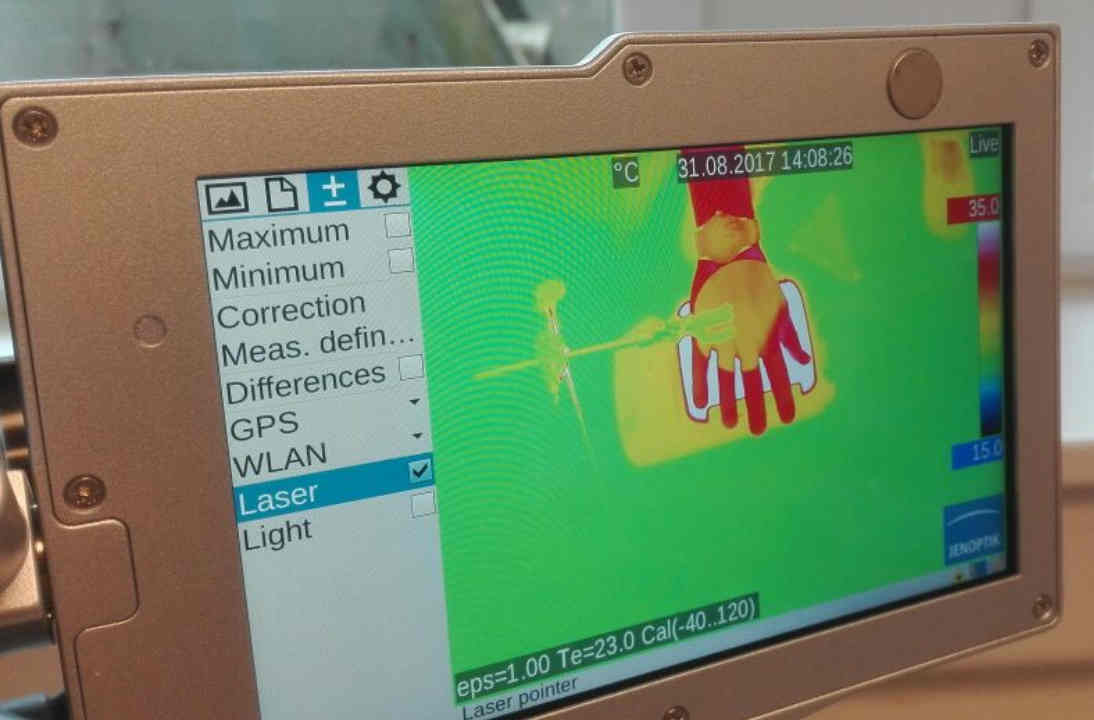
\includegraphics[scale=0.35]{Figures/Chapter04/HandTransmission.jpg}
			\caption{IR image (taken directly with the camera) of a circular piece of silicon wafer similar to the one glued on the polished side of the Petal showing the high transmissivity properties of the silicon. Behind the silicon there is a heating plate at 150\space$^{\circ}$C and in between the experimenter’s hand (we can clearly see the fingers shape through the silicon).}\label{fig4.4}
		\end{figure}
		
		\begin{figure}[ht!]
			\centering
			\captionsetup{justification=centering,margin=2cm}
			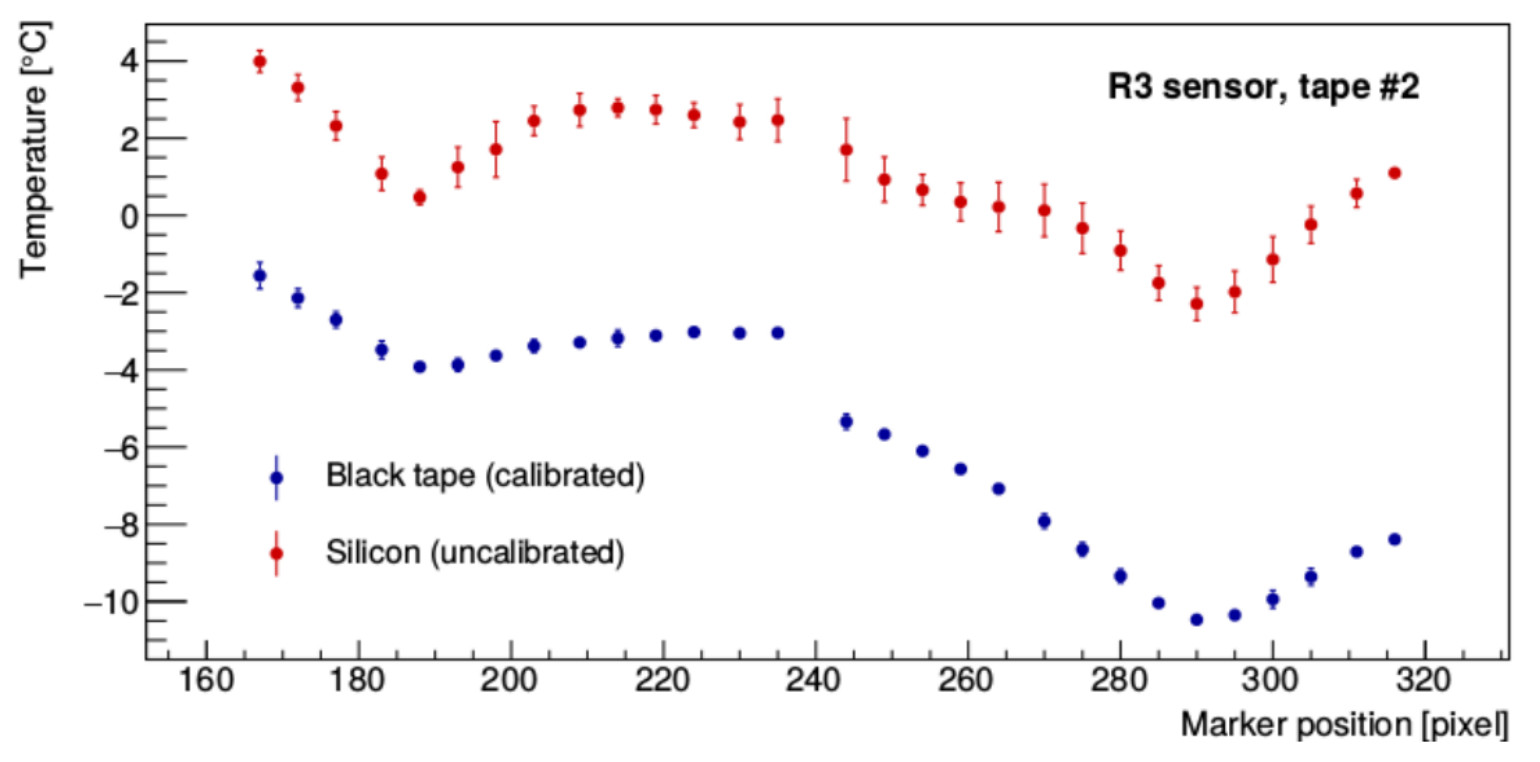
\includegraphics[scale=0.35]{Figures/Chapter04/R3Profile_Si_and_BT.jpg}
			\caption{Temperature profile plot of the second (middle) black tape strip in module R3 for the lowest temperature setpoint.}\label{fig4.5}
		\end{figure}
		
		After applying Equation \ref{eq3.3} on each pair of silicon - black tape markers and using the IRBIS software emissivity calculation tool we obtained the results shown in Figure \ref{fig4.6}. As we can see the Equation \ref{eq3.3} estimations are in good agreement with the software outputs. 
	
		\begin{figure}[ht!]
			\centering
			\captionsetup{justification=centering,margin=2cm}
			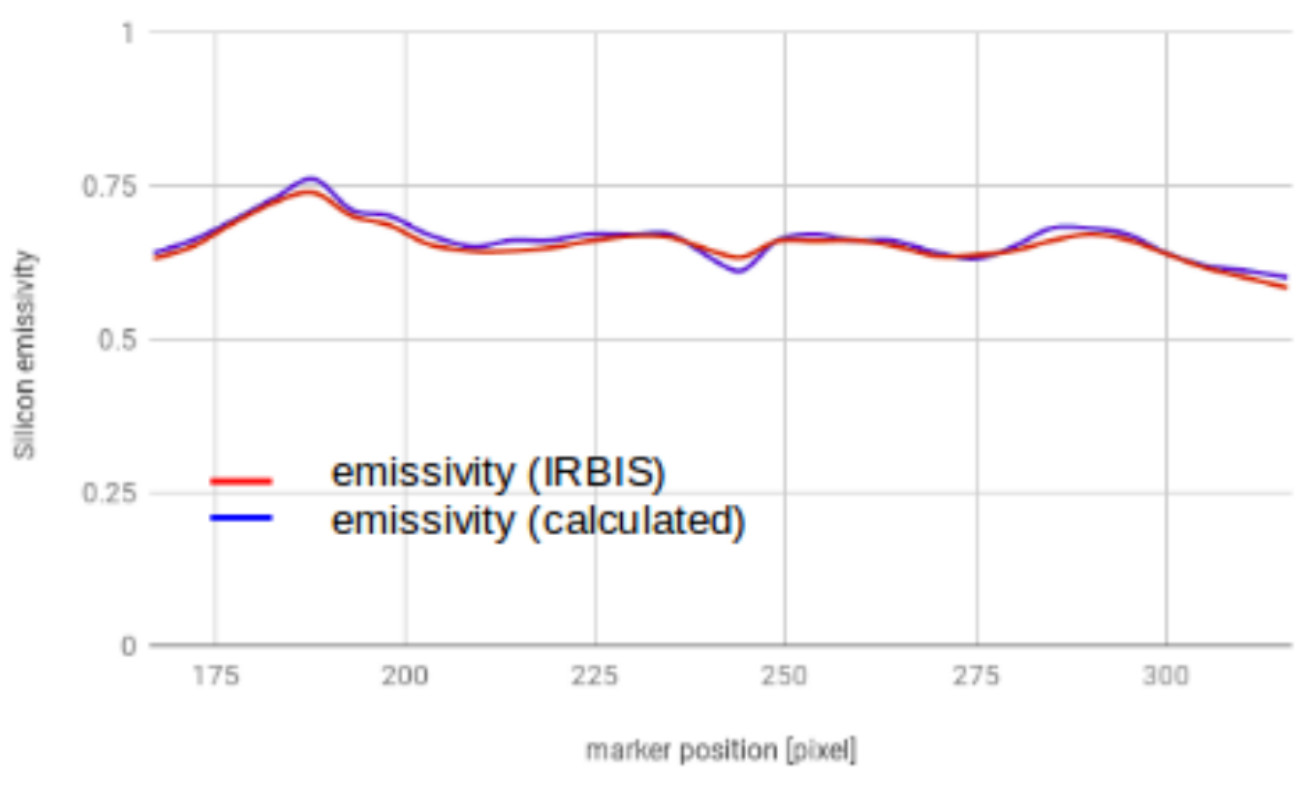
\includegraphics[scale=0.35]{Figures/Chapter04/SiliconEmissivityCalculatedVSIRBIS.jpg}
			\caption{Silicon emissivity calculated using Equation 3.3 (blue line) and the emissivity calculation tool provided by the IR camera software (red line).}\label{fig4.6}
		\end{figure}
		
		The average emissivity is estimated to be around $0.66 \pm 0.07$. By entering this value in the IRBIS software we could correct “globally” the pixels temperature to yield silicon temperatures more close to the real values. However, this would worsen the calibration for the rest of the surfaces making their temperature values to shift greatly from the truth value.\bigskip
		
	\section{IR camera spectral response scale factor.}\label{section4.4}
	
		Figure \ref{fig4.7} (left) shows the results of the estimation of the $R$ scale factor for the IR camera. The method used was described in Section \ref{section3.2}, however, to test the method’s validity we used as well a Petal thermogram of which we knew the real surface temperatures, that is, the powered off Petal at room temperature. Figure \ref{fig4.7} (right) shows the scale factor estimation on the Petal.
		
		\begin{figure}[ht!]
			\centering
			\captionsetup{justification=centering,margin=2cm}
			\includegraphics[scale=0.5]{Figures/Chapter04/BucketScaleFactors.pdf}
			\includegraphics[scale=0.5]{Figures/Chapter04/PetalScaleFactors.pdf}
			\caption{Fits of the IR camera response scale factor calculated for different temperatures (left) and using a Petal thermogram (right).}\label{fig4.7}
		\end{figure}
		
		For the calculations, the values of the black tape in silicon modules R0, R1 and R2 were used, showing consistent results with the values obtained with the aluminum bucket. The uncertainty shown is the fit’s root mean squared error. With this test we corroborated that this factor is only dependent on the IR sensor/camera and independent of the temperature and the surface.\bigskip
		
	\section{Viewing angle influence in the measurements.}\label{section4.5}
	
		In order to test whether or not the viewing angle played a significant role in the IR temperature measurements, the aluminum rod described in Section \ref{section3.4} was used, filled with water at 34.6\space$^{\circ}$C. The results can be seen in Figure \ref{fig4.8}. 
		
		We observed that the temperature variations along the rod are within 1\space$^{\circ}$C including the error bands from an angle of 0$^\circ$ (with respect to the normal of the rod’s surface) to roughly 30$^\circ$. For the central values this difference is less than 0.2\space$^{\circ}$C. This is a relatively small variation for that angular range and even though we see a drop in the markers temperature with respect to the real temperature (measured with a thermocouple directly inside the rod) the error magnitude make us conclude that, within this uncertainty, the angle influence on the IR temperature measurements is quite negligible.
		
		\begin{figure}[ht!]
			\centering
			\captionsetup{justification=centering,margin=0cm}
			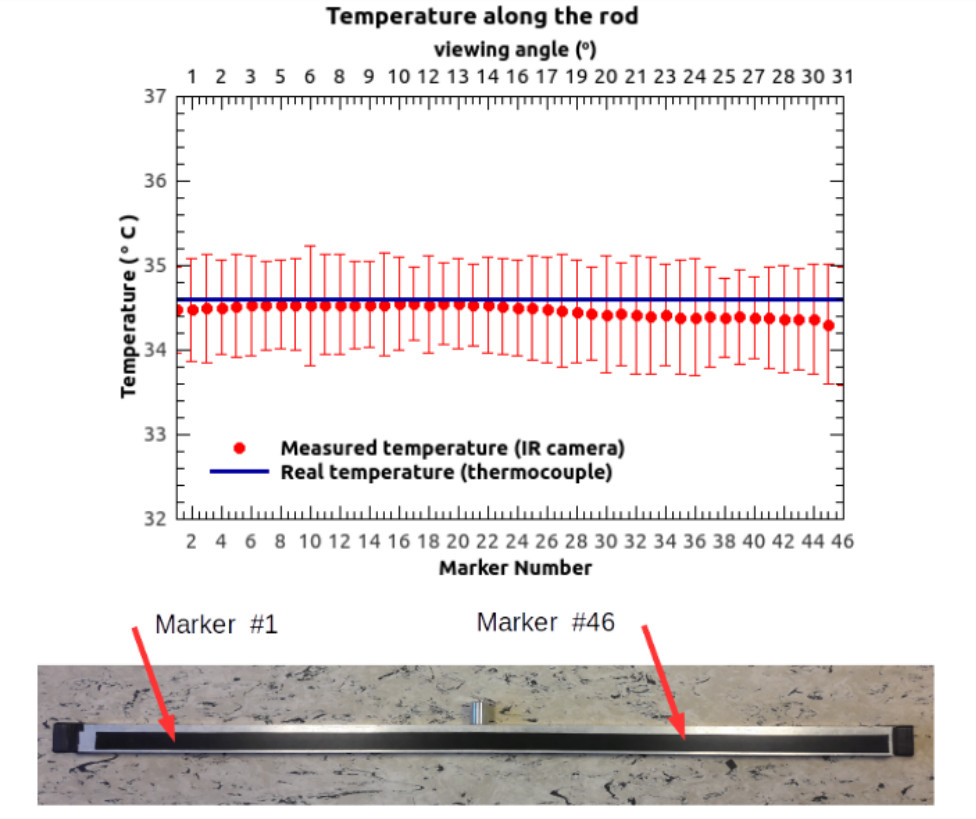
\includegraphics[scale=0.4]{Figures/Chapter04/RodAngularTempResults.jpg}
			\caption{Angle study results (top) using the aluminum rod filled with water at 34.6\space$^{\circ}$C (bottom). The marker positions do not cover the entire rod since it is larger than the Petal and some portions fall out of the viewing field of the camera.}\label{fig4.8}
		\end{figure}
	
	
	\clearpage
	
	% % % Set the style for this file:
\pagestyle{conclusions}

% % % Beginning of the section
\section*{\uppercase{Conclusions}}\label{concl}
	\bigskip
	\bigskip
	With this study, the results of the last two thermal cycles performed on the thermomechanical prototype of the petal are presented. For the first time, a $CO_{2}$ cooling system was used, which allowed us to reach lower temperatures (about -20 $^\circ_{C}$ at inlet pipe). Also, some improvements in the experimental setup related to the insolation of the thermal chamber and data acquisition procedure were adopted. Several PT100 thermocouple sensors were placed on the petal's silicon surface to obtain an alternative temperature reading to compare with the IR measurements. In general, the thermocouples readings and the camera ones (corrected using the black tape method) behave quite similar for most of the sensors. Discrepancies arise possibly related to misplacement of the PT100s are observed for a couple of sensors.\bigskip
	
	Using a set of over 560 measurement areas defined in the IRBIS software, a temperature map of the petal modules was obtained using linear interpolation. The results were compared with the results obtained with the FEA model showing some similitudes.\bigskip
	
	Emissivity of the silicon surface of the unpolished side of the petal has been estimated to be $\varepsilon=0.66\pm0.07$ by means of Equation 3.14 which is in good agreement with the values calculated using the emissivity calculation tool provided by the IR camera software. For the polished side we expect the value to be much less since the surface is highly reflective. This value allows us to globally correct the petal thermograms to show more realistic temperature values (only) on the surface of the silicon.\bigskip
	In addition, the IR camera spectral response scale factor was calculated using an alternative setup consisting in an aluminum bucket filled with water. The results were compared with the ones obtained using a petal thermogram (not powered at room temperature) showing good agreement, as expected for a magnitude only dependent of the IR sensor.\bigskip
	
	Finally, it is shown how the camera's viewing angle has no appreciable influence in the temperature measurements with this particular experimental setup. 
	
	\clearpage
	
	% % % Set the style for this file:
\pagestyle{references}

% % % Beginning of the section
\section*{\uppercase{References}}\label{referen}

	
	\clearpage
	
\end{document}